%%%%%%%%%%%%%%%%%%%%%%%%%%%%%%%%%%%%%%%%%%%%%%%%%%%%%%%%%%
%
% Doctoral Thesis Template @ The University of Manchester
% LaTeX Chapter Template
% Version 1 (23/07/2020)
% Joe Crone
%
% This template is based on:
% The University of Manchester, Presentation of Thesis Policy
% Research Office Graduate Education Team
% June 2017
% http://www.regulations.manchester.ac.uk/pgr-presentation-theses/
%
%%%%%%%%%%%%%%%%%%%%%%%%%%%%%%%%%%%%%%%%%%%%%%%%%%%%%%%%%%
\documentclass[../main.tex]{subfiles}
\begin{document}

% Title
%--------------------------------------------------------
\chapter{Photon Production by Inverse Compton Scattering}
\label{Photon_Production_by_Inverse_Compton_Scattering} % to reference use \ref{ChapterTemplate}

\section{Electron--Photon Interactions}
\label{sec:electron_photon_interactions}

While scattering interactions, specifically inverse Compton scattering interactions, are possible from all particles, the work presented here is only concerned with electron--photon interactions, the most commonly utilised form of inverse Compton scattering.  Electron--photon interactions are advantageous over other particle--photon interactions due to their low rest mass $m_{e}c^{2}$, resulting in a typically large Lorentz factor, which allows for the production of high energy photons as the scattered photon energy $E_{\gamma}$ of an ICS interaction is proportional to the Lorentz factor (Eq.~\ref{eq:Lorentz_factor}) squared ($E_{\gamma}\propto\gamma^{2}$) i.e. a double Doppler shift occurs. Within this chapter, we briefly review electron--photon interactions in general, with a focus on inverse Compton scattering, present the relevant laser physics, then extend this work to ICS photon--electron interactions on a collective basis (electron bunch--photon pulse interactions) and define several parameters to characterise the performance of radiation generation based on ICS.   

% show what happens to the electric field lines and that the kink is essentially the generated radiation (steal Hywel's diagram)
% hertzian dipole is essentially an oscillating charge (a small variation in current - charge varies locally with time)
% when a charged particle oscillates due to incident radiation or otherwise it approximates a Hertzian dipole
% continue the discussion from there + maybe show the power equation
% main results that Hywel + I went through (isotropic, polarisation conserved)
% I DEFINITELY NEED TO INCLUDE MORE MATHS + DESCRIPTION OF POWER + HOW WE GET TO THE STATEMENTS

Radiation is emitted when a charged particle is accelerated. Imagine a particle with non-zero charge $q$ is being subjected to a small, uniform acceleration $a$ for a time $\Delta t$ after which it travels at constant velocity $u=a\Delta t$ where $u\ll c$. As shown in Fig.~\ref{fig:e_field_diagram}, in the rest frame of the charged particle a radial electric field is produced however, in the laboratory frame the electric field is no longer completely radial and there is a kink corresponding to the acceleration of the charge. Note that the field lines must remain continuous because of Gauss' law in free space $\nabla\cdot\boldsymbol{E}=0$. The kink in the electric field corresponds to the emitted radiation, which is polarised in the same direction as the acceleration of the charge but emitted perpendicular to it.
\begin{figure}[!h]
\centering
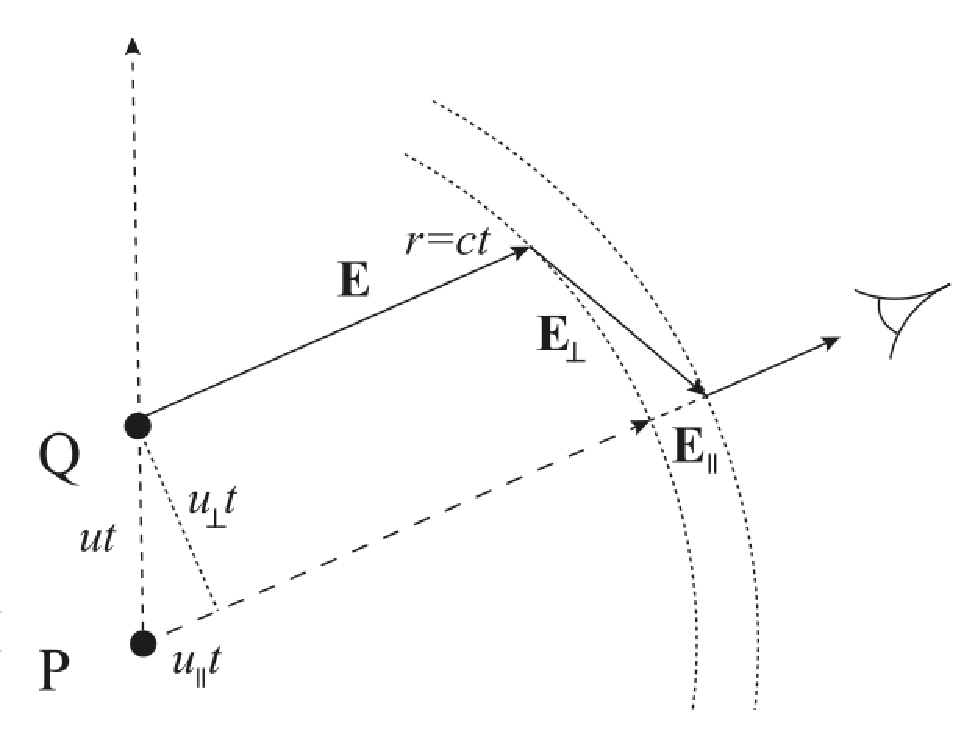
\includegraphics[width=\textwidth]{Figures/Photon_Production_by_Inverse_Compton_Scattering/E_field_diagram.pdf}
\caption{Left: A charged particle at point $P$ is uniformly accelerated to point $Q$ and then moves at constant velocity $u=a\Delta t$. An observer sees the field of the constant velocity charge within a radius $r < ct$ but when $r > ct$ the observer sees the stationary charge electric field at $P$. Since field lines must remain constant there is a kink in the electric field at $r=ct$, which corresponds to the generated radiation. Right: Isotropic electric field $\boldsymbol{E}$ of the charged particle $q$ in it's rest frame.}
\label{fig:e_field_diagram}
\end{figure}

The radial $\boldsymbol{E}_{\parallel}$ and perpendicular (kink) $\boldsymbol{E}_{\perp}$ electric fields are given by  
\begin{align}
\boldsymbol{E}_{\parallel} &= \frac{q}{4\pi\varepsilon_{0}r^{2}}, & \boldsymbol{E}_{\perp} &= \frac{qa_{\perp}}{4\pi\varepsilon_{0}c^{2}r},
\label{eq:dipole_E_fields}
\end{align}
where $\varepsilon_{0}$ is the permitivity of free space, $r$ is the radial distance and $a_{\perp}=\sin\theta$ is the perpendicular component of the uniform acceleration at an observation angle $\theta$. Hence, the magnitude of the electric field $E\left(\boldsymbol{r},t\right)$ at some location $\boldsymbol{r}$ is
\begin{equation}
\lvert\boldsymbol{E}\left(\boldsymbol{r},t\right)\rvert = \frac{q\lvert\boldsymbol{a}\left(t-r/c\right)\rvert\sin\theta}{4\pi\varepsilon_{0}c^{3}r},    
\end{equation}
and the magnitude of the magnetic field at $\boldsymbol{r}$ is $\lvert\boldsymbol{B}\left(\boldsymbol{r},t\right)\rvert = \lvert\boldsymbol{E}\left(\boldsymbol{r},t\right)\rvert/c$ because of Faraday's law. The power flow of the emitted radiation can therefore be expressed using the Poynting vector
\begin{equation}
\boldsymbol{S} = \frac{1}{\mu_{0}}\left(\boldsymbol{E}\times\boldsymbol{B}\right),
\label{eq:Poynting_vector}
\end{equation}
where $\mu_{0}$ is the permeability of free space and therefore the magnitude of the Poynting vector, the Poynting flux (power flow) becomes 
\begin{equation}
\lvert\boldsymbol{S}\left(\boldsymbol{r},t\right)\rvert = \frac{q^{2}\lvert\boldsymbol{a}^{2}\left(t-r/c\right)\rvert\sin^{2}\theta}{16\pi^{2}\varepsilonc^{3}r^{2}},
\label{eq:Poynting_magnitude}
\end{equation}
where, as expected, $P \propto 1/r^{2}$ and $P \propto \sin^{2}\theta$ which means the angular distribution of the emitted radiation is in the dipole pattern shown in Fig.~\ref{fig:dipole_angular_distribution}.
\begin{figure}[!h]
\centering
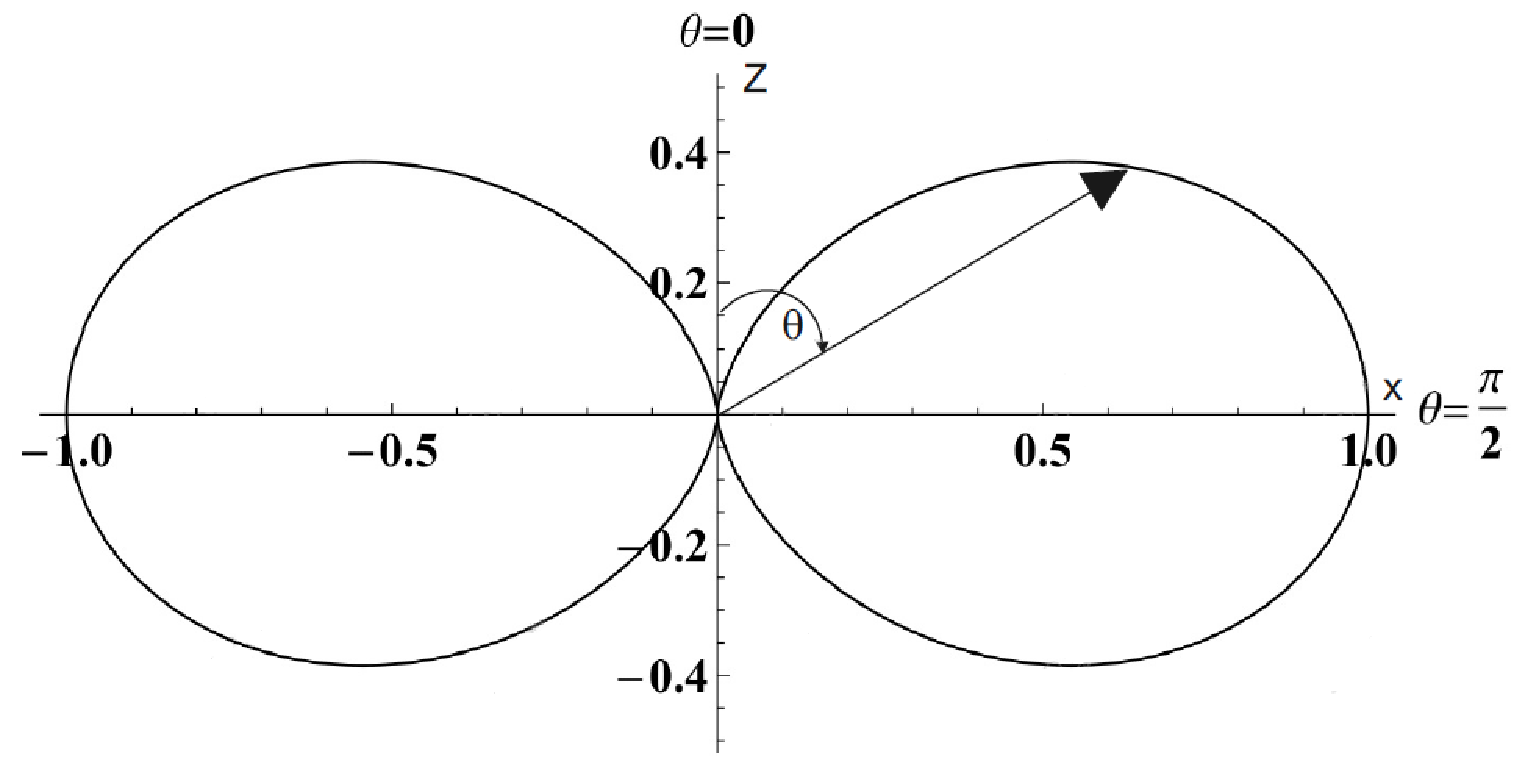
\includegraphics[width=0.7\textwidth]{Figures/Photon_Production_by_Inverse_Compton_Scattering/dipole_angular_distribution_fixed.pdf}
\caption{Angular distribution of the emitted radiation from an accelerated charge. The charge is accelerated along the $z$ axis, and hence no radiation is emitted in this direction. The distribution is the familiar dipole radiation pattern.}
\label{fig:dipole_angular_distribution}
\end{figure}
The power of the emitted radiation by an accelerated charge as a function of time can therefore be found by integrating over the emitted radiation, which occurs into a spherical surface area $\boldsymbol{A}$
\begin{equation}
P\left(t\right) = \oint\boldsymbol{S}\cdot d\boldsymbol{A} = \frac{q^{2}a^{2}\left(t-r/c\right)}{6\pi\varepsilon_{0}c^{3}},
\label{eq:accelerated_charge_radiation_power}    
\end{equation}
where $d\boldsymbol{A} = 2\pi r^{2}\sin\theta d\theta$, and (Eq.~\ref{eq:accelerated_charge_radiation_power}) is Larmor's formula. Considering an alternative scenario more appropriate to modelling radiation production, we imagine the acceleration applied to the charged particle with charge $q$ that causes the particle to oscillate over a distance $l$. This is analogous to the well-known Hertzian dipole which is comprehensively detailed in many textbooks \cite{purcell1965electricity,appleby2020science} therefore, for brevity, we instead replicate the main results. The oscillating charge causes a current $I$ to flow
\begin{equation}
I = \frac{dQ}{dt} = q\omega\cos\left(\omega t\right),    
\end{equation}
where $\omega$ is the frequency of the oscillation. Therefore, the power of the emitted radiation by Larmor's formula (Eq.~\ref{eq:accelerated_charge_radiation_power}) is
\begin{equation}
P\left(t\right) = \frac{l^{2}\omega^{2}}{6\pi\varepsilon_{0}c^{3}}q^{2}\omega^{2}\sin\left(kr-\omega t\right),
\label{eq:dipole_radiation_power}    
\end{equation}
where $k$ is the wavenumber of the emitted radiation. Consequently, the average power becomes
\begin{equation}
\langle P\rangle = \frac{q^{2}l^{2}\omega^{4}}{12\pi\varepsilon_{0}c^{3}}.   
\end{equation}
To summarise the important results: an oscillating charge emits radiation at the identical frequency to the frequency of the driver of the oscillation, the power of the emitted radiation rapidly increases with oscillation frequency ($P \propto \omega^{4}$), the emitted radiation is polarised in the direction of the applied acceleration and the angular distribution of the radiation follows the dipole radiation pattern with $P \propto \sin^{2}\theta$. Next we consider incident radiation as the cause of the acceleration applied to a charged particle. Note that within the rest of this Chapter, electrons are the only charged particle considered. 

The simplest radiation scattering interaction is Thomson scattering \cite{thomson1904xxxiv} where radiation is incident upon an electron and later scattered. The electron is treated classically because the incident radiation is much lower energy $E_{L}=hf$, with $h$ Planck's constant and $f$ the frequency, than the rest mass of the electron $m_{e}c^{2}$ ($m_{e}c^{2}\gg h\nu$). The incident radiation causes the electron to oscillate and therefore be accelerated, much like the previous Hertzian dipole case. The accelerated electron subsequently emits radiation, which is emitted isotropically in the electron frame. The radiation is emitted at an identical frequency to the incident radiation and therefore no energy is transferred; the scattering is elastic. Polarisation of the incident radiation is conserved as in the Hertzian dipole case.     

Thomson's radiation scattering model was furthered by Compton \cite{compton1923quantum}, where the scattering between a photon and an electron -- named Compton scattering -- is modelled. Here we consider a photon of momentum $\hbar k_{1}$ is incident upon a non-relativistic electron ($\gamma \ll 1$) of momentum $p_{1}$. The incident photon accelerates the electric charge as in Thomson scattering however, the incident photon recoils because momentum has been transferred from the photon to the electron. The electron is scattered with higher momentum $p_{2}$ ($p_{2}>p_{1}$) whereas the photon recoils with lower momentum $\hbar k_{2}$ ($\hbar k_{1} > \hbar k_{2}$) and consequently the scattered photon wavelength is increased relative to the incident photon wavelength. The scattering is clearly inelastic and the magnitude of the photon recoil can be expressed as $X=4E_{L}/m_{e}c^{2}$, where $E_{L}$ is the energy of the incident photon. The decrease in momentum of the photon also causes an angular dependence on the variation of the wavelength $\Delta\lambda$ as given by
\begin{equation}
\Delta\lambda = \frac{h}{m_{e}c^{2}}\left(1-\cos\theta\right),
\label{eq:Compton_wavelength}    
\end{equation}
where $\theta$ is the scattering angle of the photon with respect to the electron. As in Thomson scattering, the polarisation of the incident photon is conserved by the scattered photon. Compton scattering experiments are a fundamental proof of the particle nature of light because classical electromagnetism can't predict the observed reduction in photon wavelength.

Within this thesis, we are concerned with inverse Compton scattering -- the process of scattering a photon from a relativistically-moving electron where the scattered photon gains energy from the recoiling electron. Inverse Compton scattering was first proposed by Feenberg and Primakoff \cite{feenberg1948interaction} as a mechanism for cosmic rays to reduce in energy as they propagate throughout the universe. A simple diagram of inverse Compton scattering is shown in Fig.~\ref{fig:ICS_simple_diagram}.
\begin{figure}[!h]
\centering
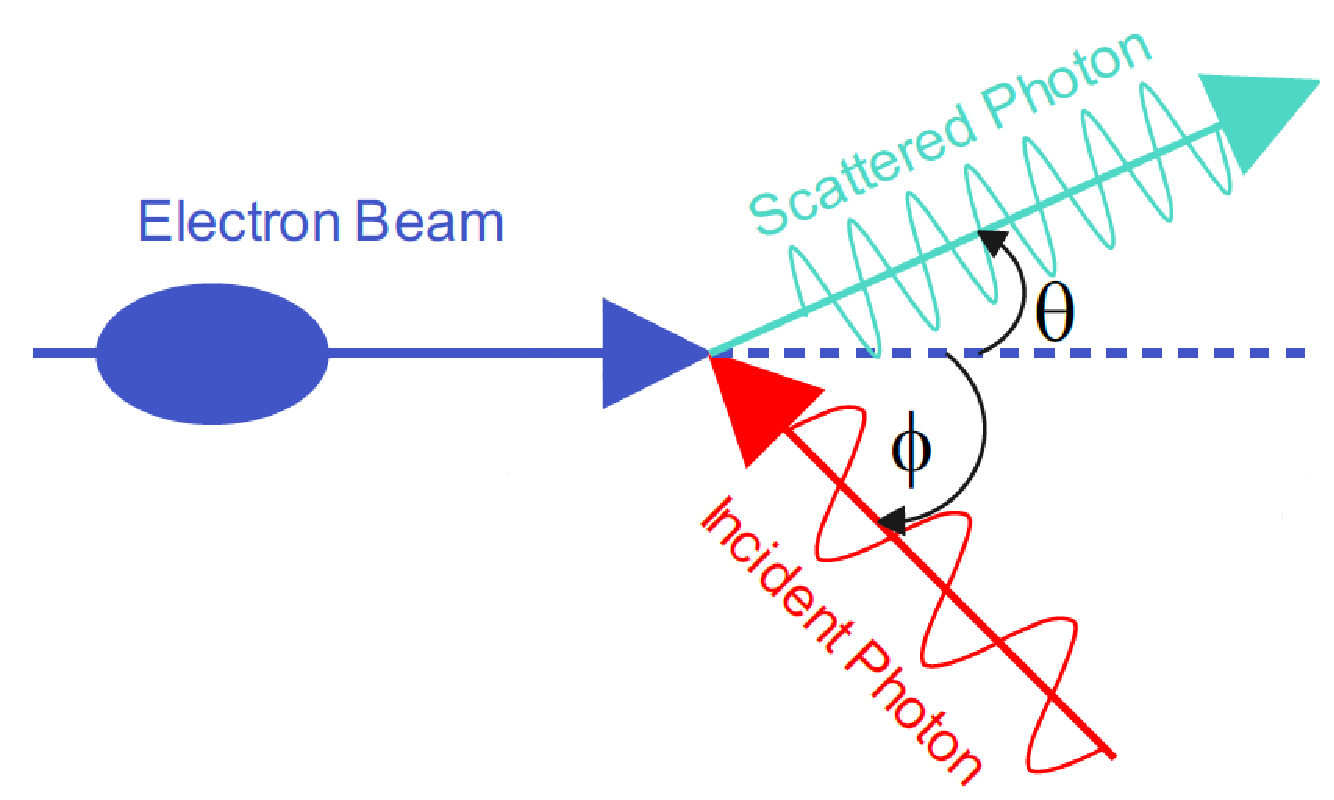
\includegraphics[width=0.6\textwidth]{Figures/Photon_Production_by_Inverse_Compton_Scattering/ICS_simple_fixed.pdf}
\caption{The inverse Compton scattering interaction where an electron beam (blue) is interacted with an incident photon (red), typically from a laser, at a crossing angle $\phi$ and scattered to higher energy (frequency) (green) at an scattering angle $\theta$. Energy is transferred from the electron beam to the scattered photon and therefore the electron beam energy is reduced.}
\end{figure}
Classically inverse Compton scattering can be understood via the changing frames of reference of the photon at different stages in the scattering process. Firstly, the incident photon is Doppler shifted into the reference frame of the electron as given by
\begin{equation}
f'=\gamma\left(1+\beta\cos\phi\right)f,    
\end{equation}
where $f'$ and $f$ are the incident photon frequency in the electron frame and lab frame respectively and $\phi$ is the crossing angle between the electron and the incident photon, as explained in Fig.~\ref{fig:scattered_photon_kinematics}. In the lab frame the photon (incident radiation) accelerates the electron and, as in the Hertzian dipole, causes the electron to oscillate and subsequently emit a photon (scattered radiation). A Lorentz transformation is then required to model the emitted radiation within the lab frame, which results in the radiation being scattered into a cone of angle $1/\gamma$ in the forward direction. The inverse Compton scattering process is often described as a double Doppler shift because the Lorentz transformation is of similar form to a Doppler shift. Again, the polarisation of the initial photon is preserved, when the electron polarisation is neglected, as in the Hertzian dipole case. Notably, once the electron is non-relativistic ($\gamma \ll 1$) there is a negligible recoil of the electron and the process tends to Thomson scattering.

However, as noted inversely for Compton scattering, the classical picture is insufficient to describe the recoil of the electron in inverse Compton scattering. Therefore, a full quantum picture is required. Photon--electron interactions can be represented with complete generality by using the two quantum electrodynamic leading order Feynman diagrams as shown in Fig.~\ref{fig:ICS_Feynman_diagrams}. 
\begin{figure}[!h]
\centering
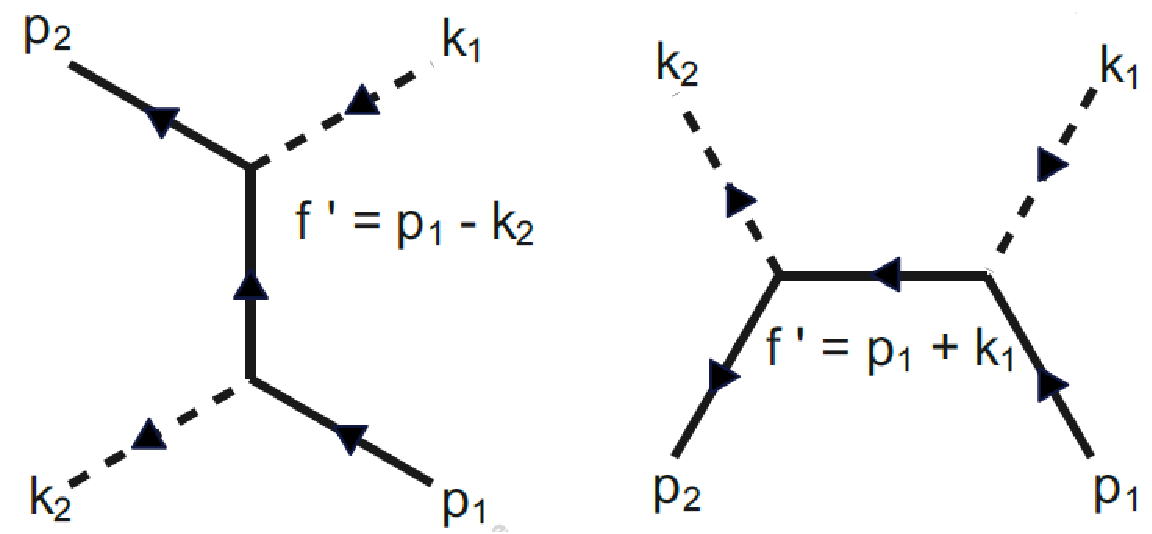
\includegraphics[width=0.65\textwidth]{Figures/Photon_Production_by_Inverse_Compton_Scattering/ICS_feynman_fixed.pdf}
\caption{Two tree-level Feynman diagrams of photon (dashed)--electron (solid) interactions, which contribute to the matrix element of the (inverse) Compton scattering process \cite{berestetskii1982quantum}. Left: The scattered photon $k_{2}$ is emitted with the annihilation of the incident electron $p_{1}$, and the incident photon $k_{1}$ is absorbed with the production of the recoiling electron $p_{2}$. Right: The incident photon $k_{1}$ and electron $p_{1}$ are absorbed, and the scattered photon $k_{2}$ is emitted with the recoiling electron $p_{2}$.}
\label{fig:ICS_Feynman_diagrams}
\end{figure}
The general form of the electron--photon interactions can be specified by
\begin{equation}
p_{1} + k_{1} = p_{2} + k_{2},
\label{eq:ICS_process}
\end{equation}
where $p_{1}$ is the four-momenta of the incident electron, $k_{1}$ is the four-momenta of the incident photon, $p_{2}$ is the four-momenta of the recoiling electron, and $k_{2}$ is the four-momenta of the scattered photon. The geometry of the inverse Compton scattering interaction in a 2D plane is shown in Fig.~\ref{fig:scattered_photon_kinematics}.
\begin{figure}[!h]
\centering
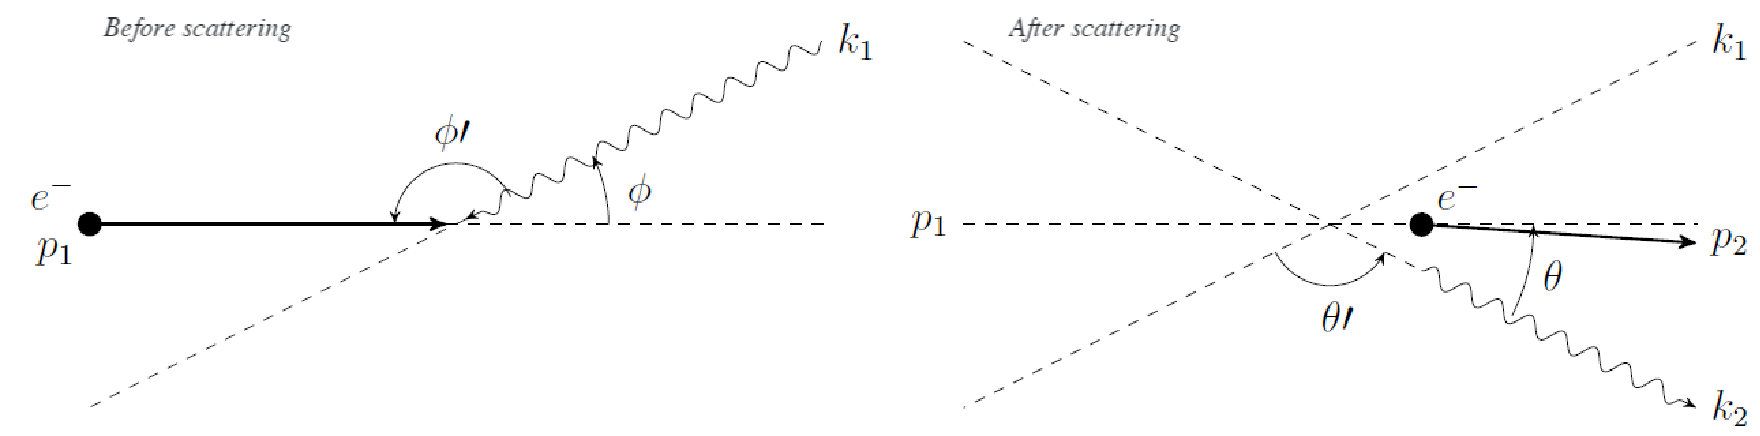
\includegraphics[width=\textwidth]{Figures/Photon_Production_by_Inverse_Compton_Scattering/scatteringkinematicsdiagram.pdf}
\caption{Geometry of the inverse Compton scattering event at the interaction point. The interaction geometry follows the geometry prescribed by Sun et al \cite{sun2009energy}. Here $\theta$ is the scattering angle of the photon, with $\phi' = \pi -\phi$, the angle between the incident electron and incident photon, where $\phi$ is the crossing angle of the electron and photon and $\theta' = \pi - \theta - \phi$ the angle between the incident and scattered photon. Left: Before interaction. Right: After interaction.}
\label{fig:scattered_photon_kinematics}
\end{figure}

Motivated by the geometry of the inverse Compton scattering process, as shown in Fig.~\ref{fig:scattered_photon_kinematics}, the initial photon $p_{1}$ and electron $k_{1}$ four-momenta can be expressed by
\begin{align}
p_{1} &= \gamma m_{e}\left(c,\boldsymbol{v_{i}}\right),
\label{eq:initial_four_vectors} \\
k_{1} &= \frac{E_{L}}{c}\left(1,\hat{n}_{i}\right), 
\end{align}
where $E_{L}$ is the energy of the incident photon, $\hat{n}_{i}$ is the unit displacement three-vector of the incident photon, $\gamma$ is the Lorentz factor, $m_{e}$ is the mass of the electron, $c$ the speed of light in a vacuum and $\boldsymbol{v_{i}}$ is the velocity three-vector of the incident electron with magnitude $v_{i}$. Similarly, we can present the final electron and scattered photon states with four-momenta
\begin{align}
p_{2} &= \gamma' m_{e}\left(c,\boldsymbol{v_{f}}\right), \\
k_{2} &= \frac{E_{\gamma}}{c}\left(1,\hat{n}_{f}\right), 
\label{eq:final_four_vectors} 
\end{align}
where $E_{\gamma}$ is the scattered photon energy, $\hat{n}_{f}$ is the unit displacement three-vector of the scattered photon, $\gamma'$ is the Lorentz factor of the recoiling electron and $\boldsymbol{v_{f}}$ is the velocity three-vector of the recoiling electron with magnitude $v_{f}$.

Using the four-momenta definitions (Eq.~\ref{eq:initial_four_vectors}-\ref{eq:final_four_vectors}), a  series of kinematic invariants (Mandelstam variables \cite{mandelstam1958determination}) can be determined for the photon-electron scattering process \cite{berestetskii1982quantum}
\begin{align}
s &= \left(p_{1}+k_{1}\right)^{2} = \left(p_{2}+k_{2}\right)^{2},
\label{eq:s_Mandelstam} \\
t &= \left(p_{1}-p_{2}\right)^{2} = \left(k_{2}-k_{1}\right)^{2},
\label{eq:t_Mandelstam} \\
u &= \left(p_{1}-k_{2}\right)^{2} = \left(p_{2}-k_{1}\right)^{2}.
\label{eq:u_Mandelstam}
\end{align}
where $t$ desribes the momentum transfer of the process, $s$ is the centre of mass energy squared and $u$ has more tenuous physical meaning, describing the cross-channel of the interaction \cite{berestetskii1982quantum}. The kinematic invariants can be used to form more convenient Lorentz invariants
\begin{align}
X &= \frac{s-\left(m_{e}c\right)^{2}}{\left(m_{e}c\right)^{2}},
\label{eq:X_Mandelstam} \\
Y &= \frac{\left(m_{e}c\right)^{2}-u}{\left(m_{e}c\right)^{2}},
\label{eq:Y_Mandelstam}
\end{align}
which, when transformed into the geometry as shown in Fig.~\ref{fig:scattered_photon_kinematics}, can be re-wrote as
\begin{align}
X &= \frac{2\gamma E_{L}\left(1+\beta\cos\phi\right)}{m_{e}c^{2}},
\label{eq:X_geometry} \\
Y &= \frac{2\gamma E_{\gamma}\left(1-\beta\cos\theta\right)}{m_{e}c^{2}},
\label{eq:Y_geometry}
\end{align}
where $\beta = v/c$ is the Lorentz speed factor.

Taking the head-on interaction case ($\phi = 0$) and assuming the incident electron is ultra-relativistic ($\beta \rightarrow 1$), the $X$ invariant simplifies to 
\begin{equation}
X = \frac{4\gamma E_{L}}{m_{e}c^{2}}.
\label{eq:X_headon}
\end{equation}
The Lorentz invariant $X$ can also be termed the recoil parameter, which denotes the magnitude of the recoil of the incident electron. For the case $X \ll 1$, the recoil is small and inverse Compton scattering reduces to Thomson scattering, the interaction becomes elastic. To illustrate, assuming a head-on interaction ($\phi=0$) with a near-infrared laser (Nd:YAG, $\lambda = 1064$~\si{\nano\meter}, see Section~\ref{sec:lasers_fabry_perot}), a 1\% recoil effect ($X = 0.01$) requires an electron kinetic energy of $E_{e} = 558$~\si{\mega\electronvolt}, via re-arrangement of (Eq.~\ref{eq:X_headon}). For a visible green wavelength ($\lambda = 532$~\si{\nano\meter}), a electron kinetic energy $E_{e} = 279$~\si{\mega\electronvolt} is required. Therefore, as the sources designed in this thesis typically use near-infrared incident photons (as explained in Section~\ref{sec:lasers_fabry_perot}), recoil effects are expected to be non-negligible only in designs for $\gamma$-ray ICS sources (where the electron beam energy is 100's~\si{\mega\electronvolt}).   

\section{Lasers and Fabry--Perot Optical Re-circulation Cavities}
\label{sec:lasers_fabry_perot}

Inverse Compton scattering sources, which use the inverse Compton scattering process to produce Doppler-shifted scattered radiation, require a source of incident photons. Ideally the incident photon beam will be monochromatic, have a high power and be of small physical dimensions upon interaction (as explained in future sections) to produce a scattered photon beam with identical characteristics. The incident photon beam criteria is satisfied for two photon sources: accelerator produced radiation, such as synchrotron radiation and free electron lasers; and lasers. Inverse Compton scattering has been demonstrated using a photon beam from an FEL as the incident photons at the HI$\gamma$S ICS source \cite{weller2009research} and synchrotron radiation has also been proposed as a source of incident photons \cite{shimada2010inverse}. Within this thesis only lasers are considered as incident photon sources for ICS sources because these are more common ICS sources, and do not require the construction of two accelerator light sources as is required for an ICS source using a photon beam from an FEL.

ICS sources can be designed using two approaches we term `single shot' and `re-circulated pulse', which relate to design of the optical system -- a schematic of each is shown in Fig.~\ref{fig:single_shot_4mirror}. In `single shot' ICS sources each incident photon pulse is used once; typically a high peak power laser pulse with up to Joule-scale laser pulse energies and pulse durations in the range 1~\si{\pico\second}--10~\si{\femto\second} is interacted with an electron bunch to scatter photons. The interaction rate (repetition rate) of the source is limited by the repetition rate of the laser pulse to the \si{\hertz} to \si{\kilo\hertz} range. In comparison re-circulated accelerators have 10--100~\si{\mega\hertz} bunch repetition rates and linear accelerators typically operate with bunch repetition rates on the \si{\kilo\hertz}-scale. Therefore, the `single shot' approach is most applicable to linear accelerators because the laser repetition rate and electron bunch repetition rate are similar. The `single shot' approach applied to a re-circulated accelerator would fail to take advantage of the high electron bunch repetition rate. As detailed in Section~\ref{sec:nonlinear_ICS}, high energy laser pulses can cause non-linear ICS interactions, which may be beneficial for some ICS source developments and is most achievable with this configuration. 
\begin{figure}[!h]
\centering
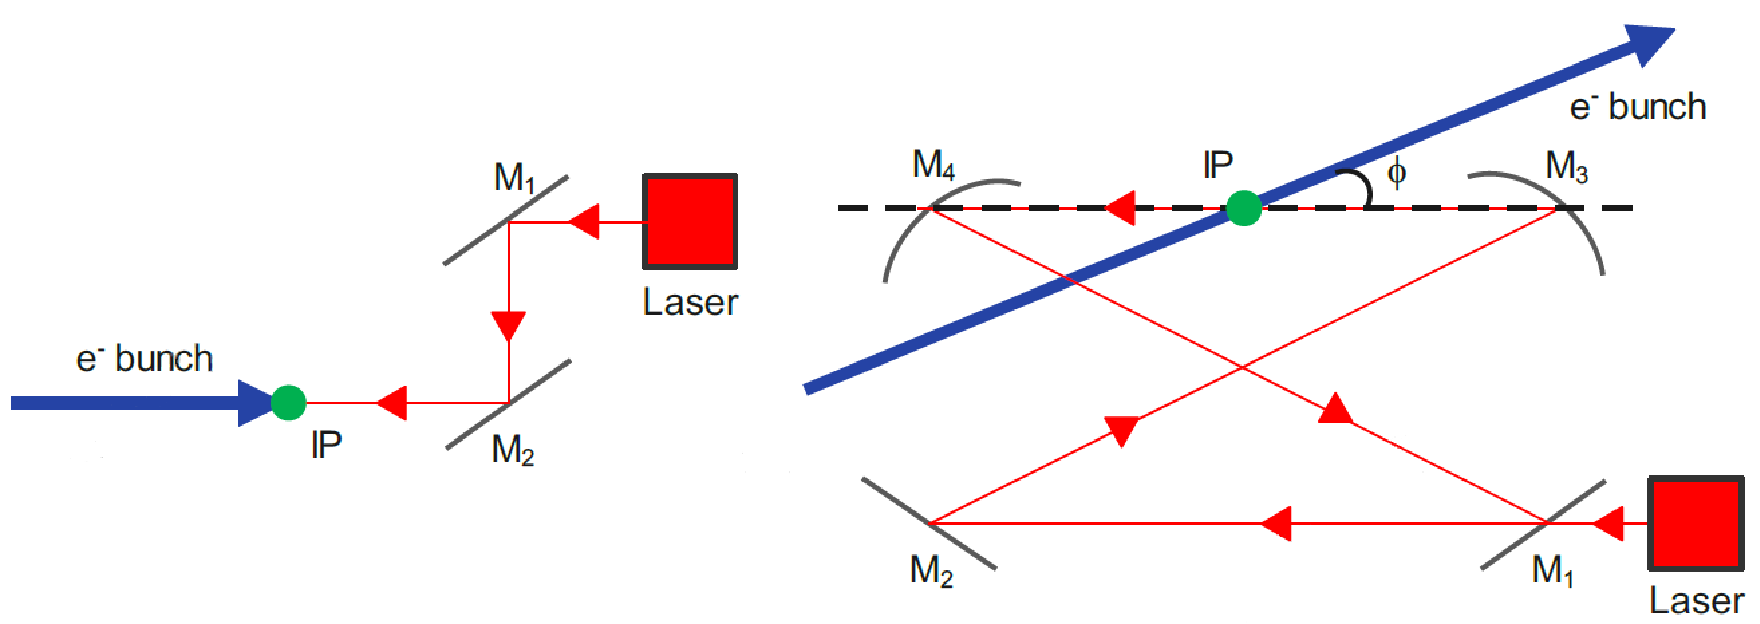
\includegraphics[width=\textwidth]{Figures/Photon_Production_by_Inverse_Compton_Scattering/single_shot_4_mirror.pdf}
\caption{Possible interaction configurations for ICS sources. Left: `Single shot' ICS source, where a laser pulse (red) is generated and interacted at the interaction point (green) in a head-on ($\phi=0$) geometry with the electron bunch (blue). Mirrors (grey) are used to transport the laser pulse to the IP. Right: `Re-circulated pulse' ICS source, where a laser pulse (red) is interacted with the electron bunch (blue) at the IP (green). The laser pulse is re-circulated by the mirrors (grey) of the optical cavity and re-interacted with the next recirculated electron bunch.}
\label{fig:single_shot_4mirror}
\end{figure}

Alternatively, the `re-circulated pulse' approach utilises a re-circulated laser pulse where a series of mirrors are used to reflect the laser pulse (or laser pulses) to the interaction point many times. Re-circulation of the laser pulse is achieved by Fabry-Perot optical cavities, detailed in Section~\ref{sec:fabry_perot_optical_cavities}. Re-circulation of the incident photon pulse enables a higher photon pulse repetition rate of around 10--100's~\si{\mega\hertz}, increasing the possible interaction frequency of the ICS source and the number of potential photon scattering events. A higher repetition rate of the laser pulse means this approach is more useful for re-circulated accelerators such as storage rings and ERLs. However, re-circulation of the laser pulse places limitations upon the laser pulse energy that may be recirculated -- Joule-scale pulse re-circulation has not been demonstrated -- which is further explored in Section~\ref{sec:fabry_perot_optical_cavities}. Non-linear ICS sources may also be excluded from the `re-circulated pulse' approach as the reduced pulse energies in re-circulated optical cavities may not achieve the intensity required for non-linear ICS.     

\subsection{Lasers for Inverse Compton Scattering Sources}
\label{sec:ICS_lasers}

Lasers providing the incident photon pulse for an ICS source are selected due to wavelength (incident photon energy), the pulse duration, the compatibility with optical mirror technologies -- high reflectivity optical mirror coatings are only available in certain wavelength regimes -- and the spectral bandwidth of the radiation. Certain lasers do not produce photons in continuous wave mode but are pulsed; continuous wave lasers and those with a higher repetition frequency can be considered for `re-circulated' pulse operation. Some lasers may only be considered for `single shot' ICS sources because of their repetition rate, though with a short pulse duration and high total energy pulses, these can still be effective ICS sources.

Many lasers may be frequency doubled (second harmonic generation) \cite{franken1961generation} where an incident photon pulse passing through a non-linear crystal material can generate a new pulse with half the incident wavelength. For example, an Nd:YAG laser may be frequency doubled to reduce the wavelength from $\lambda=1064$~\si{\nano\meter} to $\lambda=532$~\si{\nano\meter} \cite{kozlovsky1988efficient}, which has an incident photon energy of $E_{L}=2.34$~\si{\electronvolt}. However, conversion efficiency -- the efficiency in transferring power from the initial pulse to the second harmonic pulse -- can limit the pulse energy of frequency doubled lasers. Pulse durations remain unchanged from the fundamental harmonic of the Ti:Sa case and the spectral bandwidth is preserved.  

Many lasers are applicable to ICS sources and this discussion is not comprehensive, but to illustrate the above criteria we consider several laser types: CO$_{2}$ ($\lambda=10.6$~\si{\micro\meter}), Ti:Sa ($\lambda=800$~\si{\nano\meter}) , Nd:YAG ($\lambda=1064$~\si{\nano\meter}) and a frequency doubled Nd:YAG laser ($\lambda=532~\si{\nano\meter}$). Typical parameters for these laser systems are quoted in Table~\ref{tab:laser_type_parameters}.
\begin{table}[!h]
\centering
\caption{Typical laser parameters for four different laser systems commonly utilised in ICS sources.}
\vspace{3mm}
\resizebox{\columnwidth}{!}{
\begin{threeparttable}
\begin{tabular}{lccccc}
\hline\hline
Parameter & CO$_{2}$ \cite{ovodenko2016high,pogorelsky2020converting,thorlabs2021co2optics} & Ti:Sa \cite{priebe2008inverse,thorlabs2021tisaoptics} & Nd:YAG \cite{akagi2016narrow,pogorelsky2020converting,thorlabs2021ndyag200,thorlabs2021ndyagoptics} & 2nd Harmonic Nd:YAG \cite{thorlabs2021ndyagoptics} & Unit\\
\hline
Wavelength, $\lambda$ (Photon Energy, $E_{L}$) & 10600 (0.12) & 800 (1.55) & 1064 (1.17) & 532 (2.34) & \si{\nano\meter} (\si{\electronvolt})\\
Pulse Energy, $E_{\mathrm{pulse}}$ & $3\times 10^{-4}$  & 0.86~\tnote{b} & $6.2\times 10^{-5}$~\tnote{c} \cite{akagi2016narrow} & $6.2\times 10^{-5}$~\tnote{c} & \si{\joule} \\
No. Photons (100~\si{\micro\joule} Pulse) & 53.3 & 4.03 & 5.34 & 2.67 & $\times 10^{14}$ \\
Pulse Duration (\textit{rms}), $t_{\mathrm{pulse}}$ & 100~\tnote{d} & 0.08 & 5~\tnote{e} & 5~\tnote{e} & \si{\pico\second}\\
Repetition Frequency, $f_{\mathrm{laser}}$~\tnote{a} & $1.5\times 10^{4}$ & 10 & 5$\times 10^{3}$ & $5\times 10^{2}$ & \si{\hertz}\\
Spectral Bandwidth, $\Delta E_{L}/E_{L}$ & $4.95\times 10^{-4}$ & $4.42\times 10^{-2}$ & $4.7\times 10^{-4}$ & $9.4\times 10^{-4}$ & \\
Mirror Reflectivity Coefficient, $R$ & $<0.99$ & $<0.99$ \cite{thorlabs2021tisaoptics} & $<0.995$ & $<0.99$ & \\
Mirror Damage Threshold, $P/A_{\mathm{dam}}$ & 10 & 0.4~\tnote{f} & 20 & 0.55 & \si{\kilo\watt}/\si{\centi\meter}$^{2}$\\
\hline
\end{tabular}
\begin{tablenotes}
\item[a]{Repetition frequency is quoted for the laser system without a Fabry-Perot optical re-circulation cavity.}
\item[b]{Ti:Sa lasers are readily available with pulse energies up to 5~\si{\joule} but the ALICE ICS source laser \cite{priebe2008inverse} is used as an example.}
\item[c]{Nd:YAG lasers are readily available with pulse energies up to 10~\si{joule} \cite{ekspla2021ndyag} (5~\si{\joule} frequency doubled).}
\item[d]{Laser pulse durations of 5~\si{\pico\second} can be achieved by splitting this pulse into many sub-pulses \cite{pogorelsky2020converting}.}
\item{Can be operated in CW, typical pulsed operation values given.}
\item[f]{The damage threshold is quoted in units of \si{\joule}/\si{\centi\meter}$^{2}$ because a Ti:Sa laser is typically used for single shot ICS experiments, see data sheet \cite{thorlabs2021tisaoptics} for more details.}
\end{tablenotes}
\end{threeparttable}}
\label{tab:laser_type_parameters}
\end{table}

The Nd:YAG requency doubled laser, with the lowest wavelength ($\lambda=532$~\si{\nano\meter}), has the highest photon energy ($E_{L} = 2.34$~\si{\electronvolt}) and can scatter higher energy photons from a lower electron energy in comparison to the other lasers. A CO$_{2}$ laser produces the least energetic photons ($E_{L} = 0.12$) -- a factor of $\sim20$ lower -- and would require a factor of 4.5 increase in electron beam energy (Eq.~\ref{eq:scattered_photon_energy}) to scatter photons of identical energy. Therefore, production of x-ray and $\gamma$-ray radiation can be achieved more readily with Ti:Sa and Nd:YAG lasers than with CO$_{2}$ lasers.

Table~\ref{tab:laser_type_parameters} shows that, for an invariant laser pulse total energy, more photons are included in the pulse when a longer wavelength is used. A 100~\si{\micro\joule} CO$_{2}$ laser pulse ($\lambda = 10.60$~\si{\mico\meter}) contains $\sim10$ times more photons than a 100~\si{\micro\joule} Nd:YAG laser pulse ($\lambda = 1.064$~\si{\micro\meter}). More photons present in the laser pulse--electron bunch interaction linearly increases the luminosity of the ICS source as discussed in Section~\ref{sec:luminosity_and_flux} so a longer wavelength ICS source may be more intense.

A CO$_{2}$ laser also has the longest pulse duration of any laser at 100~\si{\pico\second} in comparison to the 82~\si{\femto\second} COHERENT Ti:Sa laser system \cite{priebe2008inverse}. Chirped pulse amplification (CPA) \cite{strickland1985compression} is frequently used with Ti:Sa lasers to obtain high pulse powers on the Joule-scale with short pulse durations. Short laser pulse durations, subject to the electron bunch duration, allow for generation of short duration scattered photon pulses that can be applied to experiments where phenomena occurs on femtosecond timescales. However, the picosecond domain achieved by Nd:YAG lasers is satisfactory for most experiments.

The \si{\kilo\hertz} laser repetition rates, as shown in Table~\ref{tab:laser_type_parameters} achieved by all lasers excluding Ti:Sa systems are adequate for use within the `re-circulated pulse' ICS source approach. Lasers can circulate within a Fabry-Perot cavity at 100's~\si{\mega\hertz} repetition rates but laser photons are lost in every pass of the optical cavity because mirrors aren't 100\% reflective. A \si{\kilo\hertz} repetition rate laser can be used to top up the energy of the re-circulated laser pulse and mitigate this effect, hence the Ti:Sa laser can not be used by the `re-circulated pulse' approach.

High reflectivity mirrors with reflection coefficient $R < 0.99$ are available for all of the lasers in Table~\ref{tab:laser_type_parameters} so the laser can be transported to the ICS interaction with low-losses. The reflection coefficient denotes the fraction of the incident laser power that is reflected by the mirror. However, optics for the Nd:YAG laser have demonstrated higher reflection coefficients ($R=0.995$) than other laser systems so Nd:YAG lasers can be transported in Fabry-Perot optical cavities with lower photon losses than other laser systems. Lower photon losses are advantageous because they allow a larger average photon power to be stored within the Fabry-Perot optical cavity which increases the luminosity (see Section~\ref{sec:luminosity_and_flux}) of the ICS source.

The power transported in an optical system is also limited by the damage threshold of the mirrors; a higher average stored power can be contained in a Fabry-Perot cavity if the damage threshold is increased. The damage threshold is the maximum tolerable incident laser power per unit area of the mirror. Table~\ref{tab:laser_type_parameters} shows that the Nd:YAG mirrors have the highest damage threshold of $20$~\si{\kilo\watt}/\si{\centi\meter}$^{2}$ of incident laser power per unit mirror area which means higher average laser power can be stored in a Fabry-Perot cavity using an Nd:YAG laser and these optics. Notably, the damage threshold for the 2nd harmonic Nd:YAG laser system ($\lambda = 532$~\si{\nano\meter}) is reduced by a factor of $\sim36$ compared to the fundamental Nd:YAG harmonic ($\lambda = 1064$~\si{\nano\meter}). Damage thresholds do not decrease linearly with wavelength because the damage threshold is sensitive to the particular material properties of the high reflectivity coating used to construct the optical mirror and typically development of reflective coatings has focused on the near-infrared wavelengths.  

The spectral bandwidth -- the photon energy spread of the laser pulse -- of the Nd:YAG laser system ($\lambda = 1064$~\si{\nano\meter}) is the smallest of those surveyed in Table~\ref{tab:laser_type_parameter} which is advantageous for the generation of small energy spread (bandwidth) scattered radiation, as discussed in Section~\ref{sec:bandwidth}. Scattered photons may not have a lower energy spread than the incident photons in the ICS interaction, therefore using the Ti:Sa laser ($\Delta E_{L}/E_{L} = 0.0442$) means the scattered radiation has a minimum energy spread of 4.42\%. The spectral bandwidth is increased when a laser is frequency doubled so frequency doubled lasers may be less suitable for narowband photon generation. Narrowband radiation is required for experiments that probe phenomena occurring from a small photon energy range. Consequently, a small spectral bandwidth is required for a laser used in an ICS source.   

\subsection{Fabry--Perot Optical Cavities}
\label{sec:fabry_perot_optical_cavities}

A Fabry--Perot optical cavity is a Fabry--Perot interferometer \cite{fabry1901new} utilised as an optical resonator, where incident photon pulses (laser pulses) are stacked to increase the circulating pulse energy \cite{schawlow1958infrared,variola2011luminosity}.
The Fabry-Perot optical cavity consists of a set of optical mirrors designed to transport a laser pulse with low losses and produce a small laser focus at a position within the round trip of the cavity for and electron bunch--laser pulse interaction point. The cavity is constructed from high reflectivity mirrors, however one mirror must be less reflective -- known as the input mirror -- so that the laser pulses can enter the cavity. Fabry-Perot cavities are an optical arrangement commonly applied in the `re-circulated pulse' approach to re-circulate the laser pulse many times. Commonly, Fabry-Perot optical cavities are constructed with 2 or 4 mirrors with the most prevalent topologies shown in Fig.~\ref{fig:2_mirror_4_mirror}. Cavities can be planar -- where all mirrors are in the same plane -- or non-planar where the path of the laser pulse is three-dimensional. Non-planar cavities are preferred due to polarisation considerations \cite{zomer2009polarization}, details of this are beyond the scope of the discussion here.
\begin{figure}[!h]
\centering
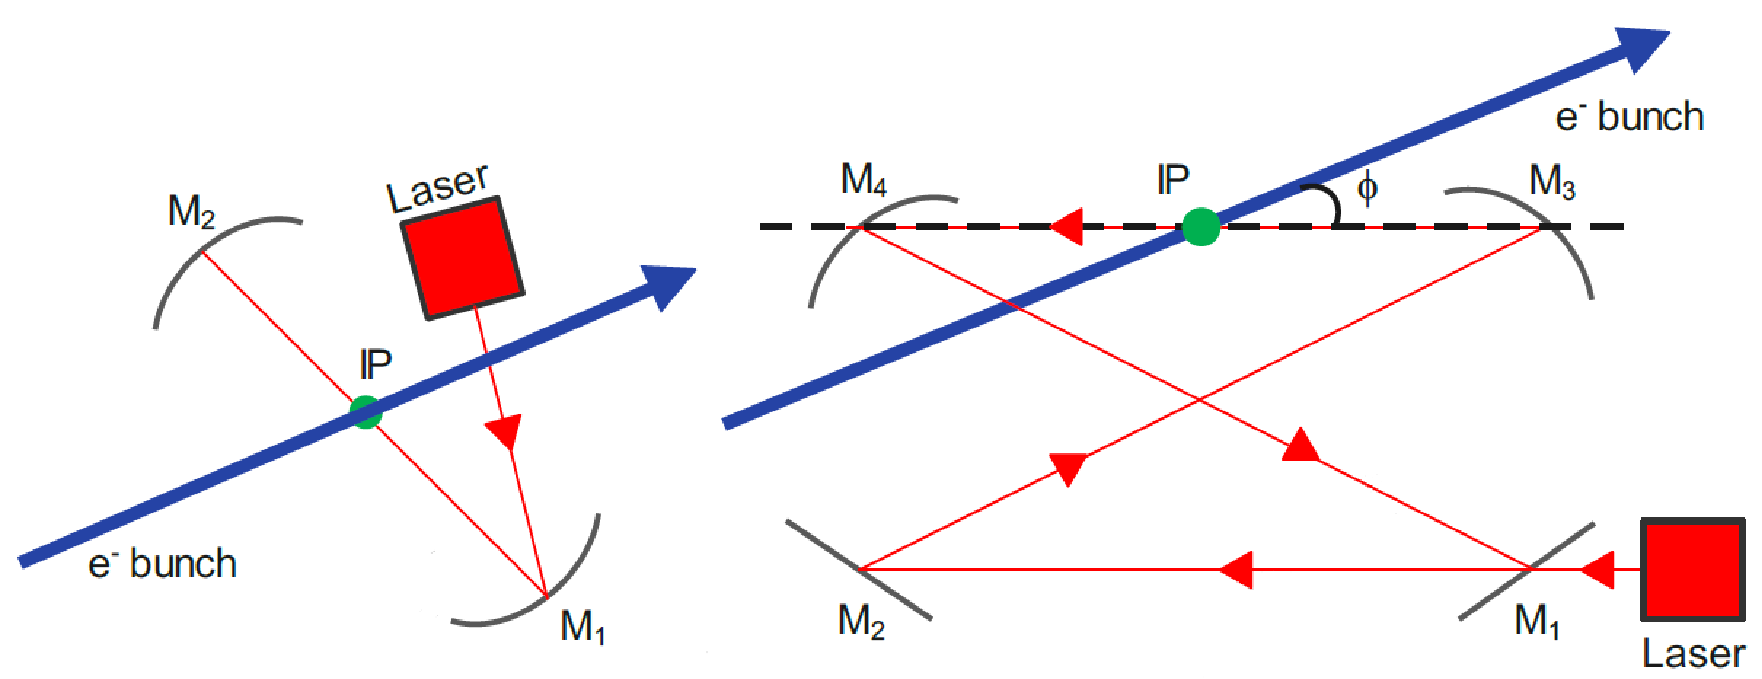
\includegraphics[width=\textwidth]{Figures/Photon_Production_by_Inverse_Compton_Scattering/2_mirror_4_mirror.pdf}
\caption{Fabry-Perot optical cavities constructed from varying amounts of mirrors (grey), where a laser (red) is circulated between the mirrors and interacted with an electron bunch (blue) at the interaction point (green) where the incident photons are scattered (light blue). At the interaction point the spot size of the laser is at a waist $\sigma_{L}$, whereas at the mirror the laser pulse has diverged and is larger, with spot size $\sigma_{w}$. Left: 2 mirror Fabry-Perot optical cavity. Right: 4 mirror bow-tie Fabry-Perot optical cavity.}
\label{fig:2_mirror_4_mirror}
\end{figure}

Two-mirror cavities consist of
two concave reflectors and require a concentric configuration to achieve a very small beam-waist where each mirror has the same focal point and the focus is at the centre of the mirrors. Consequently, the concentric configuration is mechanically very unstable \cite{dupraz2015abcd} because displacements of the optical axis
correspond to small displacement on the mirrors \cite{variola2011luminosity} -- small cavity misalignments are inherently poorly corrected by the optics. A comprehensive discussion of the mechanical instability of 2 mirror cavities and the difficulties associated with concentric configurations is presented by Zomer et al \cite{zomer2009polarization}; following the justifications of Zomer et al only 4 mirror cavities are utilised here. 

The main advantage of using a Fabry--Perot optical cavity is that the average power of the incident laser can be increased because the repetition frequency is increased from a standard laser repetition rate and the cavity can accommodate a large number of passes of the stacked optical pulse \cite{variola2011luminosity}. For example, the Nd:YAG laser in Table~\ref{tab:laser_type_parameters} has a laser repetition rate of 15~\si{\kilo\hertz}, but 100's~\si{\mega\hertz} laser pulse repetition rates can be achieved via re-circulation in an optical cavity -- a near 10,000 fold increase in laser average power. Therefore, higher average laser powers -- the stored average laser power of the cavity -- can be interacted with the high average power of a re-circulated electron bunch, with a higher interaction repetition rate, producing more inverse Compton scattering events. The average stored power of an optical cavity is given by
\begin{equation}
P_{\mathrm{avg}} = mE_{\mathrm{pulse}}f_{\mathrm{opt}},
\label{eq:average_stored_power_cavity}    
\end{equation}
where $m$ is the no. of laser pulses stored in the cavity, $E_{\mathrm{pulse}}$ is the energy of the pulse stored in the cavity and $f_{\mathrm{opt}}$ is the repetition frequency of the laser in the optical cavity. Large laser infrastructure is also not required as the Fabry-Perot optical cavity typically re-circulates weak laser pulses, with pulse energies of 10--100's~\si{\micro\joule}. High average powers can be stored as the $\sim100$~\si{\micro\joule} pulse is re-circulated at 100's~\si{\mega\hertz} -- a typical electron bunch repetition frequency -- yielding an average stored power of $P_{\mathrm{avg}}= 10$~\si{\kilo\watt}, much greater than the `single shot' approach where for Ti:Sa lasers the average power is 8.6~\si{\watt}.

However, implementation of Fabry-Perot cavities in an ICS source results in constraints to the path length of the laser pulse (denoted by the red line in Fig.~\ref{fig:2_mirror_4_mirror}), the crossing angle of the interaction, the focal radius (spot size) of the laser pulse at the interaction point and the average stored laser power available for interaction. These constraints on the optical cavity are interdependent; for example, reducing the path length will reduce the energy of the pulse that can be stored for (an assumed) invariant laser average power.

The path length constraints arise due to the requirement that the electron bunch repetition rate and the laser pulse repetition rate must remain identical. Two conditions are imposed:
\begin{align}
f_{\mathrm{electron}} &= mf_{\mathrm{opt}}, & L_{\mathrm{cav}} &= \frac{c}{f_{\mathrm{laser}}},
\label{eq:optical_path_length_conditions}    
\end{align}
where $f_{\mathrm{electron}}$ is the electron bunch repetition rate and $L_{\mathrm{cav}}$ is the path length of the cavity. A path length that is large will amplify the effect of mirror misalignments, as a ray incident on a misaligned mirror will have a larger positional error on the other cavity mirror if the distance between them is larger \cite{zomer2009polarization}. Small path lengths mean the laser spot size upon the mirrors becomes small, as the transverse \textit{rms} spot size of a laser pulse a distance $z_{L}$ from focus is given by \cite{siegmann1986lasers}
\begin{equation}
\sigma_{w} = \sigma_{L}\sqrt{1+\frac{z_{L}}{z_{R}}},
\label{eq:laser_waist}    
\end{equation}
with $\sigma_{L}$ the transverse \textit{rms} spot size of the laser pulse and the Rayleigh range \cite{siegmann1986lasers} of a laser pulse of wavelength $\lambda$ is
\begin{equation}
z_{R} = \frac{4\pi\sigma_{L}^{2}}{\lambda}.
\label{eq:rayleigh_range}    
\end{equation}
Therefore, short path lengths are unfeasible because a small laser spot size incident on a cavity mirror means the power per unit area of the laser pulse incident on cavity mirrors exceeds mirror damage thresholds (see Section~\ref{sec:ICS_lasers}).

The spot size at the interaction point of a 4 mirror cavity, as shown in Fig.~\ref{fig:2_mirror_4_mirror}, can be made smaller by increasing the distance between the two curved cavity mirrors ($M_{3}$ and $M_{4}$), whilst keeping their radius of curvature the same \cite{zomer2009polarization, akagi2016narrow}. The spot size on the $M_{3}$ and $M_{4}$ mirrors remains unchanged but, as seen through inspection of (Eq.~\ref{eq:laser_waist}), the spot size at the interaction point between these becomes smaller. Distances between the $M_{1}$ and $M_{2}$ mirrors are adjusted to maintain the path length requirements (Eq.~\ref{eq:optical_path_length_conditions}). Small laser pulse spot sizes at the IP are limited by misalignments of the optical cavity mirrors, limiting the maximum distance between the $M_{3}$ and $M_{4}$ mirrors, and the minimum distance between the $M_{1}$ and $M_{2}$ mirrors is similarly limited by the damage thresholds of those mirrors.

A crossing angle of between 2--12\si{\degree} is typically imposed between the electron bunch and the laser pulse in a Fabry-Perot optical cavity \cite{variola2011luminosity} to avoid the electron bunches hitting and causing damage to the mirror surfaces. Alternatively, two schemes could be used where a head-on ($\phi=0$) interaction is permissible:
\begin{enumerate}
    \item{The electron bunch could be incident through a hole in the mirror.}
    \item{The electron bunch could be steered into the optical cavity via a magnetic chicane (see Section~\ref{sec:magnetic_bunch_compression}). }
\end{enumerate}
When the electron bunch is incident through a hole in the mirror, the mirror itself must have a hole drilled through it. The mirror hole reduces the reflection of the cavity mirrors and consequently the stored power. Radiation damage could also occur from electron beam halo or incorrectly steered electron beams. If the electron bunch enters the Fabry-Perot optical cavity via a chicane (see Section~\ref{sec:magnetic_bunch_compression}) dipole magnets would be placed between the cavity mirrors (between M3 and M4 in the 4-mirror cavity in Fig.~\ref{fig:2_mirror_4_mirror}). These dipoles would require modification to allow a laser to pass through the magnet. Magnets within the laser path could also compromise steering of the laser beam by inducing thermal stress in the optics \cite{gunther2019device}. Induced thermal stress within the cavity optics from magnets and vibrations from vacuum equipment are two reasons Fabry-Perot cavities are difficult to implement within particle accelerators. 

The finesse of an optical cavity is defined as the number of-round trip passes a laser pulse can accomplish before being absorbed or lost by transmission through the cavity mirrors. Therefore, this is an important performance parameter of an optical cavity, analogous to the $Q$ of an RF cavity. The finesse of a Fabry-Perot optical cavity is given by \cite{ismail2016fabry}
\begin{equation}
F=\frac{\pi}{2\sin^{-1}\left(\frac{1-\sqrt{V}}{2\sqrt[4]{V}}\right)} \approx \frac{2\pi}{1-V},
\label{eq:finesse}    
\end{equation}
where $V$ is the fractional power loss per cavity round trip; the approximate form is valid for $V \ll 1$ (small round trip losses). For an input mirror with transmission $T_{1}$, the finesse becomes
\begin{equation}
F=\frac{2\pi T_{1}}{\left(T_{1}+V\right)^{2}}.
\label{eq:fabry_perot_finesse}    
\end{equation}
Consequently a high finesse cavity is necessary for transportation of a high average stored laser power; otherwise, power losses on the mirrors and mirror heating would become prohibitive. A high average power incident on a mirror heats the mirror causing thermoelastic deformation which affects the radii of curvature of the mirror. When the radii of curvature of the mirror is altered the coupling of the laser pulse to the cavity is poorer \cite{chaikovska2016high}, causing greater power loss which reinforces this behaviour until the cavity becomes unstable. Mitigation of thermoelastic deformation of optical mirrors in Fabry-Perot optical cavities is an active research subject \cite{amoudry2020modal}, where new mirror coatings could increase damage thresholds of mirrors and increase the stored laser power. A high average power also means a cavity is more susceptible to hot-spot defects, where manufacturing or handling defects on a mirror surface cause a hotspot and the mirror coating is damaged, resulting in a large loss of stored power \cite{wang2020prior}. Limitations on the average stored power within an optical cavity mean that the multi-pulse optical cavity approach (where $m$ pulses are re-circulated) is not advantageous to increasing the scattered photons produced by the ICS source because the energy of the pulses in a multi-pulse optical cavity must be decreased due to the number of pulses in the cavity i.e $E_{\mathrm{pulse}}/m$ in comparison to $E_{\mathrm{pulse}}$ for a single-pulse cavity.    

\section{Non-linear Inverse Compton Scattering}
\label{sec:nonlinear_ICS}

The inverse Compton scattering process becomes non-linear when the scattering occurs with an intense source of incident photons (intense laser pulse). The intensity of the incident photon source is typically characterised using the normalised laser vector potential $a_{0}$ defined as 
\begin{equation}
a_{0} = \frac{eE_{0}}{\omega m_{e}c} = \frac{eE_{0}\lambda}{2\pi m_{e}c^{2}},
\label{eq:a_0_momentum}    
\end{equation}
where $E_{0}$ is the amplitude of the electric field of the laser pulse and $\omega$ is the photon frequency. Therefore, the normalised laser vector potential is the ratio of the electron transverse momentum induced by the laser pulse electric field $eE_{0}/\omega$ and $m_{e}c$. Alternatively, $a_{0}$ can be represented as the ratio of the work done by the incident laser pulse over a single wavelength and the rest mass of the electron. Once $a_{0} = 1$ the transverse oscillations of the incident electron within the laser field are relativistic. The normalised laser vector potential can be more readily defined for both a longitudinally Gaussian (Eq.~\ref{eq:a0_gaussian}) and flat-top (Eq.~\ref{eq:a0_flat_top}) pulse \cite{terzic2019improving}, with a transerse Gaussian profile
\begin{align}
a_{0} &= \frac{e\sqrt{2c\mu_{0}}}{2\pi m_{e}c^{2}}\lambda\sqrt{\frac{E_{\mathrm{pulse}}}{\left(2\pi\right)^{3/2}\sigma_{L}^{2}t_{\mathrm{pulse}}}},
\label{eq:a0_gaussian} \\
a_{0} &= \frac{e\sqrt{2c\mu_{0}}}{2\pi m_{e}c^{2}}\lambda\sqrt{\frac{E_{\mathrm{pulse}}}{2\pi\sigma_{L}^{2}t_{\mathrm{pulse}}}},
\label{eq:a0_flat_top}
\end{align}
where $e$ is the charge of an electron, $\mu_{0}$ is the permeability of free space, $E_{\mathrm{pulse}}$ is the energy of the incident photon pulse, $\sigma_{L}$ is the transverse \textit{rms} spot size (radius) of the incident photon pulse and $t_{pulse}$ is the \textit{rms} pulse duration. The normalised laser potential is often expressed as $a_{0} \approx 0.855\times 10^{-9} \lambda\left[\mathrm{\mu m}\right]\sqrt{I\left[\mathrm{W/cm^{2}}\right]}$, where $I$ is the peak intensity of the incident photon pulse \cite{li2004high}.

When $a_{0} \ll 1$ the inverse Compton scattering interaction is termed linear. Beyond $a_{0}\sim 1$ non-linear effects begin to affect an inverse Compton scattering source such as harmonic generation of higher energy photons \cite{sarachik1970classical,babzien2006observation} and multi-photon inverse Compton scattering \cite{bula1996observation}. Non-linear effects can occur when $a_{0}<1$ as their onset is also driven by other factors such as pulse length and shape \cite{terzic2019improving} however an intense laser pulse $a_{0}\sim 1$ is still required. When a beam of monochromatic electrons is interacted with an intense monochromatic incident photon source (conventional laser or otherwise) we expect to see well-defined energies of the backscattered photons which occur near harmonics of the linear photon energy (when $a_{0} \ll 1$). Both harmonic generation and multi-photon inverse Compton scattering result in this scenario, and as stated by Kibble and Brown \cite{kibble1965frequency} the two are equivalent models.    

In harmonic generation, the relativistic transverse motion of the electrons within the intense incident photon field causes non-linear acceleration of the electrons which produces harmonic in the spectrum \cite{brown1964interaction, sarachik1970classical,englert1983second}. For example, a linearly polarised electron in the rest frame with momentum $p_{1}$ will be at rest before entering the laser pulse but upon entering the laser pulse will be accelerated non-linearly and will orbit in a figure-8 motion around the previous momentum value $p_{1}$ which causes the production of harmonic radiation upon Lorentz transformation to the lab frame \cite{sarachik1970classical}. Alternatively in multi-photon Compton inverse scattering, an $a_{0}\sim 1$ means that more than one photon can be involved simultaneously in an ICS interaction and therefore the central equation of the ICS interaction (Eq.~\ref{eq:ICS_process}) must be modified \cite{bula1996observation,seipt2011nonlinear}
\begin{equation}
p_{1} + \mathit{n}k_{1} = p_{2} + k_{2},
\label{eq:nonlinear_electron_photon_interaction}    
\end{equation}
where $\mathit{n}$ denotes an integer value of incident photons present in the interaction. With two or more near-identical photons interacting simultaneously, the total incident photon energy is $n E_{L}$ and the scattered photon energy becomes $\sim \mathit{n}E_{\gamma}$. However, the increased recoil
\begin{equation}
X = \frac{4\gamma E_{L}n}{m_{e}c^{2}},
\label{eq:multiphoton_recoil}    
\end{equation}
from multiple photons participating in the interaction means $E_{\gamma,n} < nE_{\gamma,1}$, where $E_{\gamma,n}$ is the scattered photon energy with $n$ incident photons and $E_{\gamma,1}$ is the scattered photon energy from a single photon.

An intense laser pulse also can cause ponderomotive broadening \cite{krafft2004spectral}, where the electron bunch is decelerated by the ponderomotive force as it enters the laser pulse and accelerated as it exits which causes a broadening in the scattered photon energies. A ponderomotive force is a force that acts upon a charged particle in an oscillating electromagnetic field in the opposing direction to the high field region, hence why the ponderomotive force pushed the electron away from the central intense region of the laser pulse. Example ponderomotive broadening calculations by Seipt et al \cite{seipt2015narrowband} have shown the bandwidth (spread of scattered photon energies) of an ICS source using an intense laser ($a_{0} = 2.83$) can be increased by around 25\% without mitigation. Whilst mitigation methods exist, such as chirping of the incident laser pulse \cite{ghebregziabher2013spectralterzic2014narrow,terzic2019improving} to mitigate ponderomotive forces experienced by the electron, these are yet to be experimentally demonstrated to the authors knowledge. Hence, intense laser and non-linear effects are avoided as we aim to demonstrate narrowband ICS sources. Unless explicitly stated, all equations within this work are derived for the linear regime as this is the regime the ICS sources presented are designed to operate. 

% Ponderomotive Broadening
%Ponderomotive broadening is a form of spectral broadening caused by the ponderomotive force of the incident photon pulse acting upon the electron bunch and varying the velocity of the electrons as they transit through the laser pulse. A ponderomotive force from a strong electric field acts upon an electron via the Lorentz force (Eq.~\ref{eq:Lorentz_force}) in the opposing direction to the high field region. During a laser pulse--electron bunch interaction, the electron is decelerated upon entering the pulse then accelerated at the exit by the ponderomotive force of the laser pulse \cite{krafft2004spectral}. The corresponding velocity shifts lead to frequency shifts in theemitted radiation, increasing the width of the observed spectrum \cite{krafft2004spectral}. The broadening effect is visible in the radiation emitted from each laser harmonic. Ponderomotive broadening is a detrimental effect to production of quasi-monochromatic high-intensity scattered photon beams, which are most favoured by radiation users.  

% Ponderomotive Broadening Mitigation
%Hence, mitigation of ponderomotive effects is an extensively studied topic \cite{ghebregziabher2013spectral,terzic2014narrow,seipt2015narrowband,rykovanov2016controlling,terzic2016combining,terzic2019improving}. Strategies to mitigate ponderomotive broadening frequently involve the `chirping' (frequency modulation) of the laser pulse, where the laser pulse shape is controlled to minimize the deceleration and acceleration of the interacted electrons. Alternatively stated, the local $a_{0}$ of the laser pulse is modulated by the shape of the pulse in order to accomplish control of the ponderomotive force \cite{terzic2019improving}.  

%The laser chirp can be produced with conventional stretcher/compressor and pulse-shaper combinations \cite{ghebregziabher2013spectral}, for example by using existing conventional laser optics or via an FEL oscillator, where the substantial bunch length of the driving electron bunches are of a length where the RF-curvature energy spread is considerable, which means that the resulting laser pulse emitted by the FEL will also be chirped \cite{ghebregziabher2013spectralterzic2014narrow,terzic2019improving}. Solutions have been derived for a range of pulse shapes and modulation schemes up to a full 3D laser pulse description \cite{terzic2019improving}, however the chirping ponderomotive broadening mitigation technique is yet to be experimentally demonstrated.

% Harmonic Generation
%Harmonic generation is the non-linear inverse Compton scattering process where the incident electron is accelerated by the electromagnetic field of the incident laser pulse. Anharmonic acceleration of the electron, as it interacts with the radiation field \cite{englert1983second}, causes non-sinusoidal transverse oscillations of the electron and induced figure-8 motion, which introduces an overall redshift in the radiation spectrum, with the concomitant emission of higher order harmonics \cite{sakai2015observation}. The electrodynamics of harmonic generation by free electrons was first described quantum mechanically by Brown and Kibble \cite{brown1964interaction,kibble1965frequency} with a following classical interpretation by Sarrachik and Schappert \cite{sarachik1970classical}. 

%The harmonic generation effect at the second harmonic was said to be demonstrated in 1983 \cite{englert1983second}, however the result appeared inconclusive. Confirmation of harmonic generation was first achieved at Brookhaven National Laboratory \cite{babzien2006observation,kumita2006observation} using a 60~\si{\mega\electronvolt} electron bunch in a head-on interaction with a CO$_{2}$ laser ($\lambda = 10.6$~\si{\micro\meter}) at a normalised laser vector potential of $a_{0} = 0.35$. The scattered photon beam generated at the BNL ATF contained both the fundamental harmonic, at an energy of $E_{\gamma} = 6.5$~\si{\kilo\electronvolt}, and the second harmonic with a peak energy of $E_{\gamma} = 13$~\si{\kilo\electronvolt}. If $a_{0}$ was larger an increasingly large red-shifting of the scattered photon energy of each harmonic \cite{kibble1965frequency,sakai2015observation} would be observable, as well as the standard recoil effect in Section~\ref{sec:electron_photon_interactions}. The doubling of the scattered photon energy arises due to the electron oscillating at double the laser frequency of the fundamental harmonic. To observe the 2nd harmonic, the fundamental harmonic must be filtered via attenuation in a silver foil \cite{babzien2006observation}, which attenuates the fundamental spectrum to a larger extent because of the lower photon energy.

%However, attenuation in the Ag foil will not completely remove the fundamental harmonic, instead the transverse profile of the filtered scattered photon beam is imaged via a luminescent screen. For the second harmonic radiation a set of two off-axis intensity peaks will be observed, unlike the fundamental harmonic which shows a central intensity peak. The double peak phenomena occurs because the $\overrightarrow{v}\times\overrightarrow{B}$ term of the Lorentz force (Eq.~\ref{eq:Lorentz_force}) of the laser pulse is comparable to the electric field term, causing an electron to oscillate in the laser field at a higher frequency, with a characteristic figure of 8 transverse motion \cite{sarachik1970classical,jackson1999classical} in the electron frame. The angular intensity distribution of the produced radiation is modified from a $\sin^{2}\theta$ dependence for the fundamental harmonic to a $\cos^{2}\theta$ dependence for the second harmonic, which upon transformation to the lab frame results in the double peak behaviour \cite{babzien2006observation}. The double intensity peaks for the second harmonic are separated by an angle $\Delta\theta = 1/\gamma$.   

% Multi-Photon Compton Scattering
%Alternatively, the non-linear inverse Compton scattering process can be described as the simultaneous interaction of multiple incident photons with an electron with the scattering interaction producing a single photon. The general equation for a multi-photon interaction, modified from (Eq.~\ref{eq:ICS_process}) \cite{bula1996observation,seipt2011nonlinear}, is

%where $\mathit{n}$ denotes an integer value of incident photons present in the interaction. With two or more near-identical photons interacting simultaneously, the total incident photon energy is $n E_{L}$ and the scattered photon energy becomes $\sim \mathit{n}E_{\gamma}$. The scattered photon energy varies from $\mathit{n}E_{\gamma}$ because of redshifting and increased recoil, as discussed previously. Demonstration of a multi-photon inverse Compton scattering source by Bula et al \cite{bula1996observation} at the Final Focus Test Beam at SLAC \cite{burke1994results} showed an inverse Compton scattering interaction with 4 incident photons, using a high intensity laser pulse. Therefore, high harmonics can be achieved via this interaction. 

%The terms harmonic generation and multi-photon ICS are used interchangeably within the literature \cite{englert1983second}, however these both appear to be an identical process. Harmonic generation is typically favoured terminology by those utilising classical methods to explain the behaviour whilst multi-photon inverse Compton scattering is used when the full quantum mechanical interpretation is used. The classical theory \cite{sarachik1970classical} allows for the coarse features of the behaviour such as the figure-8 motion of the electrons in the high field pulse and the angular distribution of emission to be understood, whilst the quantum treatment \cite{brown1964interaction,kibble1965frequency} allows the description of morel subtle features such as the spin effects of the interaction \cite{seipt2011nonlinear}.    

\section{Derivation of the Scattered Photon Energy}
\label{sec:derivation_of_the_scattered_photon_energy}

The electron--photon interaction relation (Eq.~\ref{eq:ICS_process})
\begin{equation*}
p_{1} + k_{1} = p_{2} + k_{2},    
\end{equation*}
can be modified in order to calculate the scattered photon energy of an electron--photon interaction. Using the four-momenta in (Eq.~\ref{eq:initial_four_vectors}-\ref{eq:final_four_vectors}) we can create Lorentz invariant quantities from the Minkowski norms of the four-momenta 
\begin{align}
p_{1\mu}p_{1}^{\mu} &= \gamma^{2}m_{e}^{2}\left(v^{2}-c^{2}\right) = -m_{e}^{2}c^{2},
\label{eq:lorentz_invariants1} \\
k_{1\mu}k_{1}^{\mu} &= 0.
\label{eq:lorentz_invariants2}
\end{align}
We can multiply (Eq.~\ref{eq:ICS_process}) by the four-momentum  of the scattered photon and apply (Eq.~\ref{eq:lorentz_invariants2}) the Lorentz invariant 
\begin{align}
k_{2}^{\mu}\left(p_{1\mu} + k_{1\mu}\right) &= k_{2}^{\mu}\left(p_{2\mu} + k_{2\mu}\right), \nonumber\\
k_{2}^{\mu}p_{1\mu}+k_{2}^{\mu}k_{1\mu} &= k_{2}^{\mu}p_{2\mu}.
\label{eq:apply_photon_pfinal}
\end{align}

Similarly we can construct another equation by inspecting the square of the conservation of four-momentum
\begin{align}
\left(p_{1}+k_{1}\right)_{\mu}\left(p_{1}+k_{1}\right)^{\mu} &= \left(p_{2}+k_{2}\right)_{\mu}\left(p_{2}+k_{2}\right)^{\mu}, \nonumber \\
p_{1\mu}p_{1}^{\mu}+k_{1\mu}p_{1}^{\mu}+k_{1\mu}p_{1}^{\mu}+k_{1\mu}k_{1}^{\mu} &= p_{2\mu}p_{2}^{\mu}+k_{2\mu}p_{2}^{\mu}+p_{2\mu}k_{2}^{\mu}+k_{2\mu}k_{2}^{\mu},
\label{eq:apply_conservation_squared}
\end{align}
utilising the commutation of four-vectors ($p_{\mu}k^{\mu} = k_{\mu}p^{\mu}$) and our Lorentz invariants (Eqs.~\ref{eq:lorentz_invariants1}, \ref{eq:lorentz_invariants2}) we can simplify this further 
\begin{equation}
p_{1\mu}k_{1}^{\mu} = p_{2\mu}k_{2}^{\mu}.
\label{eq:end_conservation_squared}
\end{equation}
Substituting (Eq.~\ref{eq:end_conservation_squared}) into (Eq.~\ref{eq:apply_photon_pfinal}) yields
\begin{equation}
k_{2}^{\mu}p_{1\mu}+k_{2}^{\mu}k_{1\mu} = k_{1}^{\mu}p_{1\mu}
\label{eq:substitution_four_vector}
\end{equation}
Which in three-vector notation is shown as
\begin{equation}
\frac{E_{L}E_{\gamma}}{c^{2}}\left(\hat{n}_{i}\cdot\hat{n}_{f}-1\right)+\frac{E_{\gamma}}{c}\gamma m_{e}\left(\hat{n}_{f}\cdot \boldsymbol{v_{i}}-c\right) = \frac{E_{L}}{c}\gamma m_{e}\left(\hat{n}_{i}\cdot \boldsymbol{v_{i}} -c\right)
\label{eq:three_vector_solution}
\end{equation}

However, (Eq.~\ref{eq:three_vector_solution}) should be presented in terms of the angles in Fig.~\ref{fig:scattered_photon_kinematics}. The dot products within this formula can be replaced using projections to introduce the angular dependencies
\begin{align}
\hat{n}_{i}\cdot\hat{n}_{f} &= \cos\theta',
\label{eq:projection_angle_incident_scattered_photon}\\
\hat{n}_{f}\cdot \boldsymbol{v_{i}} &= v_{i}\cos\theta,
\label{eq:projection_scattering_angle}\\
\hat{n}_{i}\cdot \boldsymbol{v_{i}} &= v_{i}\cos\phi'.
\label{eq:projection_pi_minus_crossing_angle}
\end{align}
Upon introducing the projections (Eqs.~\ref{eq:projection_angle_incident_scattered_photon}, \ref{eq:projection_scattering_angle}, \ref{eq:projection_pi_minus_crossing_angle}), (Eq.~\ref{eq:three_vector_solution}) becomes
\begin{equation}
E_{L}E_{\gamma}\left(\cos\theta'-1\right)+E_{\gamma}\gamma m_{e}c^{2}\left(\frac{v_{i}}{c}\cos\theta-1\right) = E_{L}\gamma m_{e}c^{2}\left( \frac{v_{i}}{c}\cos\phi'-1\right),
\label{eq:three_vector_solution_projections}
\end{equation}
where $E_{L}$ is the incident photon energy and $E_{\gamma}$ is the scattered photon energy. Using the Lorentz speed factor $\beta = v/c$ and the total electron beam energy $E_{e} = \gamma m_{e}c^{2}$ and re-arranging, we arrive at the general linear, recoil-corrected form for the scattered photon energy resulting from inverse Compton scattering 
\begin{equation}
E_{\gamma} = \frac{\left(1-\beta\cos\phi'\right)E_{L}}{1-\beta\cos\theta+\left(1-\cos\theta'\right)\frac{E_{L}}{E_{e}}} = \frac{\left(1+\beta\cos\phi\right)E_{L}}{1-\beta\cos\theta+\left(1-\cos\theta'\right)\frac{E_{L}}{E_{e}}},
\label{eq:scattered_photon_energy}
\end{equation}
where using the definition of the crossing angle $\phi=\pi-\phi'$, as shown in Fig.~\ref{fig:scattered_photon_kinematics}, yields a more convenient form for ICS sources.   
  
In the head-on case ($\phi=0$), the scattered photon energy (Eq.~\ref{eq:scattered_photon_energy}) can be simplified to 
\begin{equation}
E_{\gamma} = \frac{\left(1+\beta\right)}{1-\beta\cos\theta-\left(\beta-E_{L}/E_{e}\right)\cos\theta},
\label{eq:headon_scattered_photon_energy}
\end{equation}
further simplification by the small angle approximation ($\theta \ll 1$) and for an ultra-relativistic electron beam ($\beta \approx 1$) yields
\begin{equation}
E_{\gamma} \approx \frac{4\gamma^{2}E_{L}}{1+\gamma^{2}\theta^{2}+X},   
\label{eq:small_angle_scattered_photon_energy}
\end{equation}
where the recoil term $X$ is given by (Eq.~\ref{eq:X_headon}). Extending this to backscattering of the incident photon ($\theta = 0$), the scattered photon energy becomes
\begin{equation}
E_{\gamma} = \frac{4\gamma^{2}E_{L}}{1+X},
\label{eq:headon_backscattering_scattered_photon_energy}
\end{equation}
which is referred to in the literature \cite{krafft2010compton} as the Compton edge as it is the highest possible scattered photon energy from an electron--photon interaction in inverse Compton scattering. The $\gamma^{2}$ factor within (Eq.~\ref{eq:headon_backscattering_scattered_photon_energy}) is due to the double Doppler shift experienced by the incident photon as it is scattered, which is best explained using the classical picture in Section~\ref{sec:intro_ICS}. At low recoil the Compton edge energy is given by the well known relation
\begin{equation}
E_{\gamma} = 4\gamma^{2}E_{L}.
\label{eq:compton_edge_energy}    
\end{equation}

Upon inspection of the generalised ICS scattered photon energy (Eq.~\ref{eq:scattered_photon_energy}), there is an explicit dependence of the scattered photon energy $E_{\gamma}$ on the scattering angle $\theta$. The scattering angle dependence of the scattered photon energy enables scattered photon energy discrimination through specification of a maximum scattering angle the radiation can traverse. By setting a maximum scattering angle $\theta_{\mathrm{max}}$ photons with lower energy, inherently scattered at angles $\theta > \theta_{\mathrm{max}}$, will be excluded -- the produced radiation can be simply collimated.   

\section{Electron--Photon Interaction Cross Section}
\label{sec:electron_photon_interaction_cross_section}

The cross section $\sigma$ defines the probability of a specific process occurring, in this case an incident photon scattering from an incident electron within an electron bunch--laser pulse interaction. For a scattering process, the cross section can be envisioned as an effective area presented by the electron to the photon. Imagined as a ballistic collision, where a series of incident discrete photons are projected at the cross section of the electron, some photons hit the target and cause scattering whilst some miss the target and do not. Therefore, the cross section describes the proportion of scattering photons. Alternatively, the cross section can be viewed as the ratio of the incident power $P_{\mathrm{in}}$ to the radiated power $P_{\mathrm{out}}$
\begin{equation}
\sigma = \frac{P_{\mathrm{out}}}{P_{\mathrm{in}}}.
\label{eq:cross_section_power}
\end{equation}

To understand the cross section of the electron--photon interaction, the interaction must be modelled three dimensionally and considerations such as polarisation must be adequately accounted for. The co-ordinate system in Fig.~\ref{fig:scattered_photon_kinematics} can be extended to a full 3D representation in Fig.~\ref{fig:3D_coord_system}, with an incident electron $p_{1}$ parallel to the $z$-axis interacting with an incident photon $k_{1}$ travelling anti-parallel, with a crossing angle $\phi$ in the $x$-$z$ plane, scattering a photon $k_{2}$ at a polar angle $\theta$ and azimuthal angle $\phi_{f}$. Whilst the incident electron is used to set the right-handed global co-ordinate system ($x$, $y$, $z$), local right-handed co-ordinate systems can be attached to the incident photon ($\tilde{x}$, $\tilde{y}$, $\tilde{z}$), which propagates anti-parallel to the electron at a crossing angle $\phi$ ($x = -\tilde{x}\sin\phi$, $z = -\tilde{z}$), and to the scattered photon ($\tilde{x}'$,$\tilde{y}'$,$\tilde{z}'$) where the variation from the electron co-ordinate system is due to the polar scattering angle $\theta$. Polarisation directions of the incident and scattered photons is typically specified in the local co-ordinate systems.  
\begin{figure}[!h]
\centering
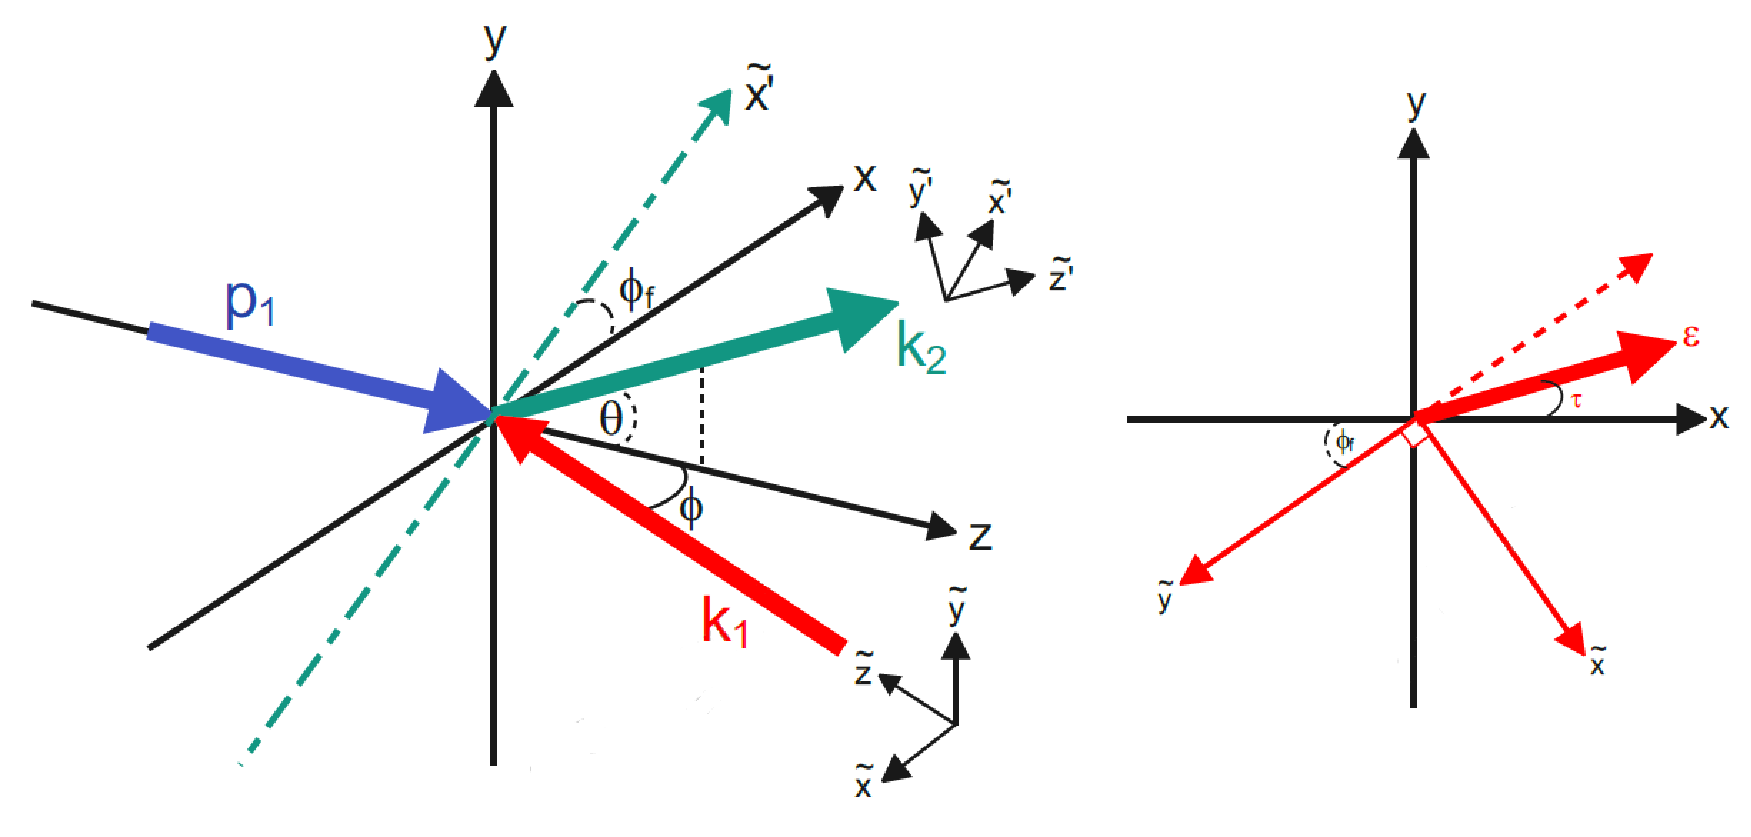
\includegraphics[width=\textwidth]{Figures/Photon_Production_by_Inverse_Compton_Scattering/ICS_interaction_polarisation.pdf}
\caption{Diagram of the electron--photon scattering interactions. Left: Geometry of the interaction in the incident electron global co-ordinate system. An incident electron (blue) with momentum $p_{1}$ interacts with an incident photon (red) with momentum $\hbar k_{1}$ at a crossing angle $\phi$ in the $x$--$z$ plane and rotated in the $x$--$y$ plane by azimuthal angle $\phi_{f}$. The photon is scattered (green) with momentum $\hbar k_{2}$ at a polar scattering angle $\theta$ in the $y$--$z$ plane with azimuthal angle $\phi_{f}$. The incident and scattered photons have local right handed co-ordinate systems attached.  Right: Polarisation vector $\varepsilon$ (red) of the incident linearly polarised photon with reference to the local co-ordinate system (red) and electron frame (black). The incident photon travels into the page, with the aximuthal angle of linear polarisation $\tau$ defined with reference to the $x$ axis of the electron frame.}
\label{fig:3D_coord_system}
\end{figure}

Following the derivation by Berestetskii, Lifshitz and Pitaevskii \cite{berestetskii1982quantum}, using the amplitude arising from the Feynman diagrams in Fig.~\ref{fig:ICS_Feynman_diagrams}, the double differential cross section with respect to any polarisation of the incident and scattered photons and an unpolarised or arbitrarily polarised electron is given by 
\begin{multline}
\frac{d^{2}\sigma}{dYd\phi_{f}} = \frac{2r_{e}^{2}}{X}\left\{\left(\frac{1}{X}-\frac{1}{Y}\right)^{2}+\frac{1}{X}-\frac{1}{Y}+\frac{1}{4}\left(\frac{X}{Y}+\frac{Y}{X}\right)  -\left(\xi_{3}+\xi_{3}'\right)\left[\left(\frac{1}{X}-\frac{1}{Y}\right)^{2}+\frac{1}{X}-\frac{1}{Y}\right] \right.\\\left. +\xi_{1}\xi_{1}'\left(\frac{1}{X}-\frac{1}{Y}+\frac{1}{2}\right) + \xi_{2}\xi_{2}'\left[\frac{1}{4}\left(\frac{X}{Y}+\frac{Y}{X}\right)\left(1+\frac{2}{X}-\frac{2}{Y}\right)\right] \right.\\\left. + \xi_{3}\xi_{3}'\left[\left(\frac{1}{X}-\frac{1}{Y}\right)^{2}+\frac{1}{X}-\frac{1}{Y}+\frac{1}{2}\right] \right\},
\label{eq:polarisation_differential_cross_section}    
\end{multline}
where the incident photon pulse Stokes parameters $\xi_{i} \left(i=1,~2,~3\right)$, in the electron frame (global) co-ordinate system, are given by
\begin{align}
\xi_{1} &= P_{t}\sin\left(2\tau-2\phi_{f}\right)\sin\phi, \\
\xi_{2} &= P_{c}, \\
\xi_{3} &= -P_{t}\cos\left(2\tau-2\phi_{f}\right)\sin\phi,
\label{eq:incident_stokes_parameters}    
\end{align}
where, using the same co-ordinate system as Sun and Wu \cite{sun2009characterizations,sun2011theoretical}, $-1 \geq P_{t} \geq 1$ is the degree of linear polarisation of the incident pulse ($P_{t}=-1$, full anti-parallel polarisation), $-1 \geq P_{c} \geq 1$ is the degree of circular polarisation of the incident pulse ($P_{c}=-1$, full anticlockwise polarisation), $\tau$ is the azimuthal angle of the linear polarisation, $\phi_{f}$ is the azimuthal scattering angle, $\phi$ is the crossing angle in the $x$--$z$ plane. Polarisation of the incident photon is shown diagramatically in Figure~\ref{fig:3D_coord_system}. The $\xi_{1}$ parameter resembles linear polarisation along the transverse axes whereas the $\xi_{3}$ parameter corresponds to linear polarisation at a 45\si{\degree} angle to the transverse axes and $\xi_{2}$ resembles to the degree of circular polarisation. For example, a linearly polarised incident photon oriented in the horizontal $x$ plane would be given by $\xi_{i} = \left(1,~0,~0\right)$ whilst $\xi_{i} = \left(0,~1,~0\right)$ describes a circularly polarised incident photon propagating clockwise. 

The Stokes parameters $\xi'_{i} \left(i=1,~2,~3\right)$ of a single scattered photon  for a small polar scattering angle ($\theta \ll 1$) in the electron frame can be similarly defined
\begin{align}
\xi'_{1} &\approx -\bar{\xi'_{1}}\cos\left(2\phi_{f}\right)+\bar{\xi'_{3}}\sin\left(2\phi_{f}\right), \\
\xi'_{2} &\approx \bar{\xi'_{2}}, \\
\xi'_{3} &\approx -\bar{\xi'_{1}}\sin\left(2\phi_{f}\right)-\bar{\xi'_{3}}\cos\left(2\phi_{f}\right),
\end{align}
where $\bar{\xi'_{i}}$ are the scattered photon Stokes parameters of the scattered photon in its attached local co-ordinate system. For example $\bar{\xi'_{i}} = \left(-1,~0,~0\right)$, corresponds to a horizontally polarised scattered photon aligned to $\tilde{y}$. For a beam of unpolarised electrons scattering with a polarised laser pulse, the polarisation of the scattered photons is parallel to the incident photon. However, since the photons can be scattering at angle $\theta$, the polarisation with respect to the scattered photon $\tilde{z}$ axis varies. 

Assuming, for the purposes of a general cross section formula,  scattered photons are not discriminated on the basis of polarisation from an ICS interaction (all scattered photon polarisations are accepted) the cross section can be derived by setting $\xi_{i}' = 0, \left(i=1,~2,~3\right)$ and multiplying (Eq.~\ref{eq:polarisation_differential_cross_section}) by 2. This is equivalent to summing over all possible polarisation states \cite{sun2009characterizations}. Making this assumption, the double differential cross section (Eq.~\ref{eq:polarisation_differential_cross_section}) reduces to
\begin{equation}
\frac{d^{2}\sigma}{dYd\phi_{f}} =  \frac{4r_{e}^{2}}{X^{2}}\left[1+P_{t}\cos\left(2\tau-2\phi_{f}\right)\right]\left\{\left(1-\xi_{3}\right)\left[\left(\frac{1}{X}-\frac{1}{Y}\right)^{2}+\frac{1}{X}-\frac{1}{Y}\right]+\frac{1}{4}\left(\frac{X}{Y}+\frac{Y}{X}\right)\right\},
\label{eq:double_differential_cross_section}    
\end{equation}
Integrating over the full range of the azimuthal scattering angle $0 \leq \phi_{f} \leq 2\pi$ obtains the differential cross section as a function of the $Y$ Lorentz invariant (Eq.~\ref{eq:Y_geometry}) 
\begin{align}
 \frac{d\sigma}{dY} &= A\int_{0}^{2\pi}1+P_{t}\cos\left(2\tau-2\phi_{f}\right)\sin\phi~d\phi_{f}+ B\int_{0}^{2\pi}~d\phi_{f}, \nonumber \\
 \frac{d\sigma}{dY} &= 2\pi\left(A+B\right) = \frac{8\pi r_{e}^{2}}{X^{2}}\left[\left(\frac{1}{X}-\frac{1}{Y}\right)^{2}+\frac{1}{X}-\frac{1}{Y}+\frac{1}{4}\left(\frac{X}{Y}+\frac{Y}{X}\right)\right],
\label{eq:differential_cross_section_Y_invariant}
\end{align}
where $A$ and $B$ collect parameters that are independent of the azimuthal scattering angle in (Eq.~\ref{eq:double_differential_cross_section})
\begin{align}
A &= \frac{4r_{e}^{2}}{X^{2}}\left[\left(\frac{1}{X}-\frac{1}{Y}\right)^{2}+\frac{1}{X}-\frac{1}{Y}\right], \nonumber\\
B &= \frac{4r_{e}^{2}}{X^{2}}\left[\frac{1}{4}\left(\frac{X}{Y}+\frac{Y}{X}\right)\right].
\label{eq:phif_independent_parameters}
\end{align}
Through inspection of (Eq.~\ref{eq:differential_cross_section_Y_invariant}), it is clear there is no longer a dependence on the polarisation of the incident photon therefore, the flux of an ICS interaction is independent of the polarisation of the incident photons.

Following the derivation of Berestetskii \cite{berestetskii1982quantum}, the Mandelstam variables for the electron--photon interaction (Eqs.~\ref{eq:s_Mandelstam}, \ref{eq:t_Mandelstam}, \ref{eq:u_Mandelstam}) are limited by $s\geq m_{e}c^{2}$, $t \leq 0$ and $u s \leq \left(m_{e}c^{2}\right)^{2}$
\begin{align}
s\geq& m_{e}c^{2}, & t \leq& 0, & us \leq& \left(m_{e}c^{2}\right)^{2},   \label{eq:mandelstam_limits} 
\end{align}
where the limit on $s$ (Eq.~\ref{eq:s_Mandelstam}) arises when the electron and photon momentum are zero, but the electron is still of rest mass $m_{e}c^{2}$. The $t$ variable (\ref{eq:t_Mandelstam}) must be smaller than zero because $p_{1}=p_{2}$ for an elastic interaction and when the electron recoils and the scattered photon gains energy $p_{1}>p_{2}$. The $us$ limit (Eq.~\ref{eq:mandelstam_limits}) is more nuanced, but also occurs because of the limit of an elastic collision and is derived more readily by Berestetskii et al \cite{berestetskii1982quantum}. The limits on the Mandelstam variables (Eq.~\ref{eq:mandelstam_limits}) can be re-arranged to form the inequality $X/X+1 \leq Y \leq X$ \cite{sun2009characterizations}. The total cross section for the inverse Compton scattering interaction \cite{berestetskii1982quantum} can be integrated within the range of the inequality
\begin{align}
\sigma &= \frac{8\pi r_{e}^{2}}{X^{2}}\int_{\frac{X}{X+1}}^{X}\left(\frac{1}{X}-\frac{1}{Y}\right)^{2}+\frac{1}{X}-\frac{1}{Y}+\frac{1}{4}\left(\frac{X}{Y}+\frac{Y}{X}\right)~dY, \nonumber \\
\sigma &= \frac{2\pi r_{e}^{2}}{X}\left[\frac{1}{2}+\frac{8}{X}-\frac{1}{2\left(1+X\right)^{2}}+\left(1-\frac{4}{X}-\frac{8}{X^{2}}\right)\ln{\left(1+X\right)}\right],
\label{eq:compton_cross_section}
\end{align}
where $r_{e}$ is the classical radius of the electron. If, as in Curatolo et al \cite{curatolo2017analytical}, we take the classical limit ($X \to 0$) of the total cross section (Eq.~\ref{eq:compton_cross_section}) we obtain
\begin{equation}
\lim_{X \to ~0} \sigma = \frac{8\pi r_{e}^{2}}{3}\left(1-X\right) = \sigma_{T}\left(1-X\right),
\label{eq:compton_cross_section_classical_limit}
\end{equation}
where $\sigma_{T}$ is the Thomson cross section. When the interaction is firmly in the classical regime ($X \ll 1$), in which inverse Compton scattering becomes Thomson scattering and there is elastic scattering, the Compton cross section recovers the Thomson scattering cross section, $\sigma = \sigma_{T}$. If we take the limit where all the energy of the incident electron is transformed to the scattered photon, where the incident electron has maximal recoil ($X \to \infty$), the cross section (Eq.~\ref{eq:compton_cross_section}) becomes
\begin{equation}
\lim_{X \to ~\infty} \sigma = \frac{2\pi r_{e}^{2}}{X}\left(\ln{X}+\frac{1}{2}\right)
\label{eq:compton_cross_section_ultrarelativistic_limit}
\end{equation}
which is known as the ultra-relativistic limit \cite{curatolo2017analytical}. At the ultra-relativistic limit the scattered photon energy (Eq.~\ref{eq:scattered_photon_energy}) approaches the incident electron energy ($E_{\gamma}\sim E_{e}$).
\begin{figure}[!h]
\centering
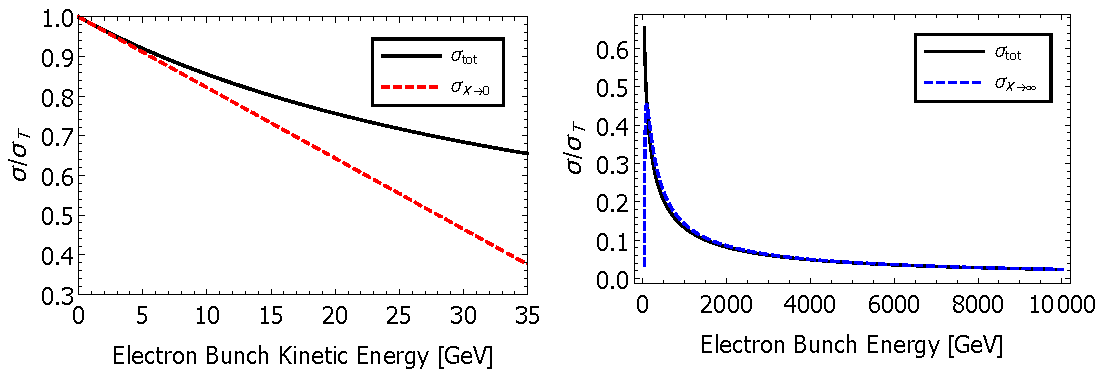
\includegraphics[width=\textwidth]{Figures/Photon_Production_by_Inverse_Compton_Scattering/Cross_Section_Electron_Bunch_Energy_NDYAG.pdf}
\caption{Electron--photon interaction cross section (Eq.~\ref{eq:compton_cross_section}) as a function of electron bunch energy for an Nd:YAG laser operating at the fundamental harmonic ($\lambda = 1064$~\si{\nano\meter}, $E_{L} = 1.17$~\si{\electronvolt}). Left: Comparison of the full cross section (Eq.~\ref{eq:compton_cross_section}) (black) with the cross section in the low recoil limit (Eq.~\ref{eq:compton_cross_section_classical_limit}) (red) for a 5~\si{\mega\electronvolt}--35~\si{\giga\electronvolt} electron bunch kinetic energy range. Right: Comparison of the full cross section (Eq.~\ref{eq:compton_cross_section}) with the cross section in the ultra-relativistic, high recoil limit (Eq.~\ref{eq:compton_cross_section_ultrarelativistic_limit}) (blue) for a 35~\si{\giga\electronvolt}--10~\si{\terra\electronvolt} electron bunch kinetic energy range.}
\label{fig:cross_section_electron_energy}
\end{figure}

The behaviour of the total cross section as a function of electron bunch energy is shown in Fig.~\ref{fig:cross_section_electron_energy}, with the low-recoil (Eq.~\ref{eq:compton_cross_section_classical_limit}) and ultra-relativistic (Eq.~\ref{eq:compton_cross_section_ultrarelativistic_limit}) limits shown. A small recoil ($X \ll 1$) cross section calculation is valid up until the \si{\giga\electronvolt}-scale, above the \si{\giga\electronvolt}-scale the small recoil approximation (Eq.~\ref{eq:compton_cross_section_classical_limit}) underestimates the electron--photon interaction cross section (Eq.~\ref{eq:compton_cross_section}). The ultra-relativistic cross section approximation (Eq.~\ref{eq:compton_cross_section_ultrarelativistic_limit}) becomes a good approximation to the full cross section calculation (Eq.~\ref{eq:compton_cross_section}) beyond  $\sim92$~\si{\giga\electronvolt}, at smaller energies the cross section is underestimated and at energies on the order of 100's~\si{\giga\electronvolt} the cross section in the ultra-relativistic approximation is negative which is clearly non-physical.     

Assuming a head-on ($\phi=0$) interaction in the ultra-relativistic domain ($\beta\approx1$) the Lorentz invariants can be related as
\begin{equation}
Y = X\frac{E_{e}-E_{\gamma}}{E_{e}-E_{L}},
\label{eq:lorentz_relation_headon_backscatter}
\end{equation}
where the derivative of $Y$ with respect to scattered photon energy becomes
\begin{equation}
\frac{dY}{dE_{\gamma}} = -\frac{X}{E_{e}-E_{L}}.
\label{eq:differential_lorentz_relation_headon_backscatter}
\end{equation}
The derivative of $Y$ with respect to the scattered photon energy $E_{\gamma}$ (Eq.~\ref{eq:differential_lorentz_relation_headon_backscatter}) is substituted into (Eq.~\ref{eq:double_differential_cross_section}), which is integrated over the azimuthal angle, similarly to (Eq.~\ref{eq:differential_cross_section_Y_invariant}), to obtain the differential cross section with respect to the scattered photon energy
\begin{equation}
\frac{d\sigma}{dE_{\gamma}} = \frac{8\pi r_{e}^{2}}{X\left(E_{e}-E_{L}\right)}\left[\left(\frac{1}{X}-\frac{1}{Y}\right)^{2}+\frac{1}{X}-\frac{1}{Y}+\frac{1}{4}\left(\frac{X}{Y}+\frac{Y}{X}\right)\right].
\label{eq:differential_cross_section_ICS_energy}    
\end{equation}

Since the differential cross section can be expressed in terms of the scattered photon energy (Eq.~\ref{eq:scattered_photon_energy}), there is a cross section--scattering angle correspondence indirectly resulting from the scattered photon energy (Eq.~\ref{eq:scattered_photon_energy}). The scattered photon energy--scattering angle correspondence is explained in Section~\ref{sec:derivation_of_the_scattered_photon_energy} and is further discussed with reference to the cross section in Section~\ref{sec:analytical_collimated_flux}. The cross section--scattering angle correspondence from the scattered photon energy is also convoluted with the scattering angle dependency of the $Y$ Lorentz invariant (Eq.~\ref{eq:Y_geometry}). A full treatment of collimation and the differential cross section with respect to scattering angle is included in Chapter~\ref{Optimisation_and_Characterisation_of_Inverse_Compton Scattering_Spectra}, where the angular solutions are used to derive an analytical model for the collimated flux of an ICS interaction.    
The scattered photon energy differential cross section (Eq.~\ref{eq:differential_cross_section_ICS_energy}) can be plotted against the scattered photon energy of a single particle ICS interaction to reveal the spectral characteristics of an ICS source. Fig.~\ref{fig:cross_section_scattered_photon_energy} shows a normalised plot of the scattered photon energy differential cross section (Eq.~\ref{eq:differential_cross_section_ICS_energy}) as a function of the scattered photon energy for a head-on collision ($\phi=0$), in the low recoil regime ($X \ll 1$). Several features are apparent in Fig.~\ref{fig:cross_section_scattered_photon_energy}, such as the double peaked spectrum -- which is peaked in the forward (low energy) and backward (high energy) directions with respect to the incident photon pulse -- where the intensity of these peaks is double (for $X \ll 1$) the intensity of the trough at $\theta=1/\gamma$ and the average energy ($E_{\gamma} = 2\gamma^{2}E_{L}$), which is half of the maximum energy (Eq.~\ref{eq:compton_edge_energy}) at the Compton edge.   
\begin{figure}[!h]
\centering
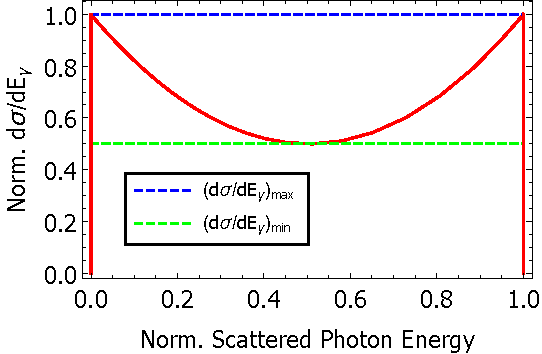
\includegraphics[width=0.6\textwidth]{Figures/Photon_Production_by_Inverse_Compton_Scattering/Cross_Section_Scattered_Photon_Energy.pdf}
\caption{Normalised differential cross section with respect to the scattered photon energy (Eq.~\ref{eq:differential_cross_section_ICS_energy}) as a function of normalised scattered photon energy (Eq.~\ref{eq:scattered_photon_energy}) in the low recoil ($X \ll 1$) regime for a head-on interaction ($\phi=0$); both parameters are normalised for generality. The maximum (blue) and minimum (green) values of the differential cross section (Eq.~\ref{eq:max_min_differential_cross_section_ICS_energy}) are shown, which differ by a factor of $\sim2$ (Eq.~\ref{eq:max_min_cross_section_ratio}).The average energy in the spectrum is $E_{\gamma}=2\gamma^{2}E_{L}$, half of the Compton edge energy (Eq.~\ref{eq:compton_edge_energy}), due to the symmetry of the spectrum.}
\label{fig:cross_section_scattered_photon_energy}
\end{figure}

The Lorentz $Y$ invariant can be calculated for the angular limitations of the ICS interaction ($0 \leq \theta \leq 1/\gamma$) -- a cone of angular width $\theta=1/\gamma$ in the backscattered direction. Taking the lower limit of $\theta = 0$ provides the minimum value of $Y$ where $Y \approx X/\left(1-X\right)$ and the scattered photon energy is given by (Eq.~\ref{eq:headon_backscattering_scattered_photon_energy}). At the large scattering angle limit $\theta = 1/\gamma$, $Y$ is at a minimum and has a value of $Y = X/\left(1-X/2\right)$ and the scattered photon energy becomes
\begin{equation}
E_{\gamma} = \frac{2\gamma^{2}E_{L}}{1+X},
\label{eq:angular_limit_scattered_photon_energy}
\end{equation}
as seen in Fig.~\ref{fig:cross_section_scattered_photon_energy}, therefore $Y = X\left(1-X/2\right)$. Substituting the limitations of the $Y$ Lorentz invariant for each angular case into (Eq.~\ref{eq:differential_cross_section_ICS_energy}) yields maximum and minimum values of the differential cross section as shown by Sun et al \cite{sun2011theoretical}
\begin{align}
\left(\frac{d\sigma}{dE_{\gamma}}\right)_{\mathrm{max}} &= \frac{8\pi r_{e}^{2}}{X\left(E_{e}-E_{L}\right)}\frac{2+X}{4}, \nonumber \\
\left(\frac{d\sigma}{dE_{\gamma}}\right)_{\mathrm{min}} &= \frac{8\pi r_{e}^{2}}{X\left(E_{e}-E_{L}\right)}\frac{1}{4\left(1+X\right)}.
\label{eq:max_min_differential_cross_section_ICS_energy}    
\end{align}
The ratio of the maximum and minimum of the differential cross section given by 
\begin{equation}
\frac{\left(d\sigma/dE_{\gamma}\right)_{\mathrm{max}}}{\left(d\sigma/dE_{\gamma}\right)_{\mathrm{min}}} = \left(2+X\right)\left(1+X\right) \approx 2,
\label{eq:max_min_cross_section_ratio}
\end{equation}
shows that the intensity of the radiation emission in the backscattered direction, at the Compton edge ($\theta=0$), is double the intensity than in the angular limit, at a semi-angle of $\theta=1/\gamma$, which is also highlighted in Fig.~\ref{fig:cross_section_scattered_photon_energy}. Furthermore, following Sun et al \cite{sun2011theoretical} by taking the small recoil limit of the cross section (Eq.~\ref{eq:compton_cross_section_classical_limit}) with (Eq.~\ref{eq:max_min_differential_cross_section_ICS_energy}), the ratio of the cross section in an energy range $\Delta E_{\gamma}$ around the Compton edge energy $E_{\gamma}^{\mathrm{max}}$ (Eq.~\ref{eq:compton_edge_energy}) in the case of low recoil ($X \ll 1$) is given by
\begin{equation}
\frac{\Delta\sigma}{\sigma} \approx \frac{3\left(2+X\right)}{4\left(1-X\right)}\frac{\Delta E_{\gamma}}{E_{\gamma}^{\mathrm{max}}} \approx \frac{3}{2}\frac{\Delta E_{\gamma}}{E_{\gamma}^{\mathrm{max}}},
\label{eq:cross_section_factor}    
\end{equation}
which can be used to estimate the part of the photon spectrum selected by a collimator aperture placed downstream of an ICS source. A full calculation of this `collimated flux' is developed in Chapter~\ref{Optimisation_and_Characterisation_of_Inverse_Compton Scattering_Spectra}, building upon the flux derivation in the next section and the cross section in (Eq.~\ref{eq:double_differential_cross_section}). 

\section{Luminosity and Flux}
\label{sec:luminosity_and_flux}

\subsection{Luminosity}

Applying Larmor's theorem \cite{larmor1897lxiii,purcell1965electricity} in the relativistic generalization \cite{jackson1999classical} and following the derivation by Krafft and Priebe \cite{krafft2010compton}, the luminosity of an ICS source in the head-on ($\phi=0$) case can be derived. Larmor's theorem of radiated power in the relativistic generalisation is 
\begin{equation}
P_{rad} = \frac{\gamma^{4}e^{2}\sigma}{6\pi \epsilon_{0}c^{3}}\lvert\dot{\boldsymbol{v}}\rvert^{2} = \gamma\sigma\epsilon_{0}c\lvert\left(\boldsymbol{E}+\boldsymbol{v}\times\boldsymbol{B}\right)\boldsymbol{x}\left(t\right)\rvert^{2},
\label{eq:larmor_formula}    
\end{equation}
where $e$ is the charge of an electron, $\epsilon_{0}$ is the permittivity of free space, $\lvert\dot{\boldsymbol{v}}\rvert$ is the acceleration of the electron in the laboratory frame, $\sigma$ is the cross section of the electron--photon interaction (Eq.~\ref{eq:compton_cross_section}) as derived in Section~\ref{sec:electron_photon_interaction_cross_section}, $\boldsymbol{E}$ and $\boldsymbol{B}$ are respectively the electric field and magnetic flux density of the incident laser, $\boldsymbol{v}$ is the velocity of the electron as it traverses the laser pulse and $\boldsymbol{x}\left(t\right)$ is the first order approximation of the trajectory of the electron as it traverses the incident laser pulse. 
Following Krafft and Priebe \cite{krafft2010compton}, the total energy radiated by the electron $U_{e^{-}}$ in a single electron--plane wave photon pulse interaction is given by 
\begin{equation}
U_{e^{-}} = \int P\left(t\right)dt = \gamma^{2}\left(1+\beta\right)^{2}\sigma\epsilon_{0}c\int\lvert\boldsymbol{E}\left(x,y,\left[\beta+1\right]ct\right)\rvert^{2}dt,
\label{eq:electron_radiated_energy}
\end{equation}
where the energy density of a plane wave laser is $\epsilon_{0}\lvert\boldsymbol{E}\rvert^{2}$. To generalise the single electron--plane wave photon pulse interaction to the energy radiated by an electron bunch--photon pulse interaction $U_{\gamma}$, we must replace the energy density of a plane wave laser by the energy density distribution of a laser pulse and convolve this with an electron bunch intensity distribution. For a head-on case $\left(\phi=0\right)$, with the laser pulse Doppler shifted into the electron frame, the radiated energy of a Gaussian electron bunch--laser pulse interaction is    
\begin{equation}
U_{\gamma} = \gamma^{2}\left(1+\beta\right)\sigma E_{L}\int c\left(1+\beta\right) n_{e}\left(\boldsymbol{r},\boldsymbol{p},t\right)n_{L}\left(\boldsymbol{r},\boldsymbol{k},t\right) d\boldsymbol{p}~d\boldsymbol{k}~dV~dt,
\label{eq:total_interaction_energy}
\end{equation}
where $n_{e}\left(\boldsymbol{r},\boldsymbol{p},t\right) = N_{e}f_{e}\left(\boldsymbol{r},\boldsymbol{p},t\right)$ is the  electron bunch intensity function as a function of the displacement vector $\boldsymbol{r}$ (integrated over volume $V$), momentum vector $\boldsymbol{p}$ and time $t$ with $N_{e}$ the number of electrons per bunch and $n_{L} = N_{L}f_{L}\left(\boldsymbol{r},\boldsymbol{k},t\right)$ is the intensity distribution of the laser pulse where $N_{L}$ is the number of photons in the incident laser pulse and $f_{L}\left(\boldsymbol{r},\boldsymbol{k},t\right)$ is the laser pulse intensity function as a function of the displacement vector $\boldsymbol{r}$, momentum vector $\boldsymbol{k}$ and time $t$. Within this derivation, the laser pulse and electron bunch are approximated by Gaussian intensity distributions, however any model such as flat-top laser pulses or Lorentzian distributed electron bunches could be substituted. The Gaussian intensity distributions of the electron bunch and laser pulse are given by \cite{sun2011theoretical}
\begin{gather} % has to be gather to fit
f_{e}\left(\boldsymbol{r},\boldsymbol{p},t\right) = \frac{1}{\left(2\pi\right)^{3}\epsilon_{x}\epsilon_{y}\sigma_{p}\sigma_{z,e}}\exp\left[-\frac{\gamma_{x}x^{2}+\alpha_{x}xx'+\beta_{x}x'^{2}}{2\epsilon_{x}}-\frac{\gamma_{y}y^{2}+2\alpha_{y}yy'+\beta_{y}y'^{2}}{2\epsilon_{y}}\right.\\\left.-\frac{\left(p-p_{0}\right)^{2}}{2\sigma_{p}^{2}}-\frac{\left(z-ct\right)^{2}}{2\sigma_{z,e}^{2}}\right], \nonumber
\label{eq:electron_gaussian_intensity_distribution} \\
f_{L}\left(\boldsymbol{r},\boldsymbol{k},t\right) = \frac{1}{4\pi^{2}\sigma_{z,L}\sigma_{k}\sigma_{w}^{2}}\exp\left[-\frac{x_{L}^{2}+y_{L}^{2}}{2\sigma_{w}^{2}}-\frac{z_{L}+ct}{2\sigma_{z,L}^{2}}-\frac{\left(k-k_{0}\right)}{2\sigma_{k}^{2}}\right],
\label{eq:laser_gaussian_intensity_distribution}
\end{gather}
where $\epsilon_{x/y}$ is the emittance of the electron beam in the $x$ and $y$ directions (see Section~\ref{sec:twiss_emittance}), $\sigma_{p}$ is the fractional momentum spread of the electron bunch, $\sigma_{z,e}$ is the \textit{rms} electron bunch length, $\beta_{x/y}$, $\alpha_{x/y}$ and $\gamma_{x/y}$ are the Twiss parameters (see Section~\ref{sec:twiss_emittance}) in either the $x$ or $y$ direction, $x$ and $y$ are the positions of the electron in both directions, similarly $x'$ and $y'$ are the angular divergences in each direction, $p$ is the magnitude of the momentum of an individual electron and $p_{0}$ is the centroid electron momentum of the bunch. The pulse length of the laser pulse is $\sigma_{z,L}$, $\sigma_{k}$ is the fractional momentum spread of the incident laser pulse, $x_{L}$, $y_{L}$ and $z_{L}$ are the positions of an incident photon in each direction, $k$ is the wavenumber of an individual photon and $k_{0}$ is the centroid wavenumber of the laser pulse and $\sigma_{w}$ is the \textit{rms} transverse waist of the laser pulse given by the usual Gaussian optics formula (Eq.~\ref{eq:laser_waist}).

The head-on Gaussian luminosity of the interaction can then be separated from the other terms in (Eq.~\ref{eq:total_interaction_energy}), assuming the interaction takes place at the waists of both pulse and bunch, by splitting the spatial terms from the energy spread terms in the electron bunch (Eq.~\ref{eq:electron_gaussian_intensity_distribution}) and laser pulse (Eq.~\ref{eq:laser_gaussian_intensity_distribution}) of the intensity functions
\begin{align}
f_{e}\left(\boldsymbol{r},\boldsymbol{p},t\right) &= f_{e}\left(\boldsymbol{r},t\right)f_{e}\left(\boldsymbol{p}\right), \\  
f_{L}\left(\boldsymbol{r},\boldsymbol{k},t\right) &= f_{L}\left(\boldsymbol{r},t\right)f_{L}\left(\boldsymbol{k}\right).
\label{eq:spartial_energy_term_split}
\end{align}
The luminosity of the head-on interaction becomes
\begin{align}
\mathcal{L}_{\mathrm{HEAD-ON}} &= N_{e}N_{L}c\left(1+\beta\right)\int f_{e}\left(\boldsymbol{r},t\right)f_{L}\left(\boldsymbol{r},t\right)~dV~dt, \\
\mathcal{L}_{\mathrm{HEAD-ON}} &= \frac{N_{e}N_{L}}{2\pi\sqrt{\sigma_{x,e}^{2}+\sigma_{x,L}^{2}}\sqrt{\sigma_{y,e}^{2}+\sigma_{y,L}}} = \frac{N_{e}N_{L}}{2\pi\sigma_{x}\sigma_{y}},
\label{eq:headon_luminosity}
\end{align}
where $\sigma_{i}(i=x,y,z) = \sqrt{\sigma_{i,e}^{2}+\sigma_{i,L}^{2}}$ is the convolution of the laser pulse and electron bunch spot sizes at the IP. The energy spread terms of the electron bunch and laser pulse (spectral bandwidth) have been neglected in (Eq.~\ref{eq:headon_luminosity}) because these have already been adequately taken into account by using the average cross-section $\sigma$, which already encapsulates the variation in number of interactions due to energy variations and because they are typically small ($\Delta E_{e}/E_{e} < 0.01$, $\Delta E_{L}/E_{L} < 0.01$). The luminosity in (Eq.~\ref{eq:headon_luminosity}) is analogous to particle collider luminosity \cite{herr2006concept,miyahara2008luminosity}, reflecting the electron--photon collider analogy of ICS sources.

\subsection{Flux}

The flux (photons generated per second) of an ICS source can be derived from the radiated energy of the ICS source and the average scattered photon energy of the emission. Using the luminosity (Eq.~\ref{eq:headon_luminosity}), the energy radiated by the interaction of a Gaussian laser pulse and electron bunch becomes  
\begin{equation}
U_{\gamma} = \gamma^{2}\left(1+\beta\right)\sigma\frac{N_{e}N_{L}}{2\pi\sigma_{x}\sigma_{y}}E_{L},
\label{eq:total_interaction_energy_simplified}
\end{equation}
which omits the hourglass effect of the two diverging beams and is also only true in the case of a head-on interaction at the waists of the laser pulse and electron bunch -- these two effects are accommodated in Section~\ref{sec:geometric_luminosity_reduction}. The solutions for each of these cases is covered in the next section. The number of photons produced per interaction $N_{\gamma}=\sigma\mathcal{L}$ can be found using the average scattered photon energy $\gamma^{2}\left(1+\beta\right)\hbar\omega$, where if $\beta=1$, $E_{\gamma} = 2\gamma^{2}E_{L}$, as shown in Fig.~\ref{fig:cross_section_scattered_photon_energy} 
\begin{equation}
N_{\gamma} = \sigma\frac{N_{e}N_{L}}{2\pi\sigma_{x}\sigma_{y}}.
\label{eq:no_photon_headon}
\end{equation}
The total flux of the photons is given by $\mathcal{F} = \sigma\mathcal{L}f$ where $\mathcal{L}$ is the luminosity of the source and $f$ is the repetition frequency of the ICS interaction. Therefore, the often quoted result \cite{krafft2010compton,curatolo2017analytical}, of the flux in the head-on configuration can be obtained
\begin{equation}
\mathcal{F} = \frac{\sigma N_{e}N_{L}f}{2\pi\sigma_{x}\sigma_{y}}.
\label{eq:headon_flux}
\end{equation}
Using the result derived in Section~\ref{sec:electron_photon_interaction_cross_section} (Eq.~\ref{eq:cross_section_factor}) for the portion of the scattered photon energy within an energy range $\Delta E_{\gamma}$ from the Compton edge (Eq.~\ref{eq:compton_edge_energy}), we can approximate the flux in a part of the ICS spectrum. For example, the flux in a 0.1\% bandwidth of an ICS source (see Section~\ref{sec:bandwidth}), in the head-on ($\phi=0$), low recoil ($X \ll 1$) case is given by
\begin{equation}
\mathcal{F}_{0.1\%} = \frac{3}{2}\times 10^{-3} \mathcal{F},
\label{eq:flux_0.1_bandwidth}    
\end{equation}
where the $3/2$ factor originates from (Eq.~\ref{eq:cross_section_factor}), the $10^{-3}$ is due to the 0.1\% bandwidth scaling and $\mathcal{F}$ is the flux (Eq.~\ref{eq:headon_flux}) of an ICS source. The flux in a 0.1\% bandwidth (Eq.~\ref{eq:flux_0.1_bandwidth}) is an important quantity for analysing the performance of an ICS source as a light source because it quantifies the portion of flux of most use for narrowband experimentation and it is used to calculate the brilliance, as expanded upon in Section~\ref{sec:peak_average_brilliance}. 

\subsection{Geometric Luminosity Reduction and Corrected Flux}
\label{sec:geometric_luminosity_reduction}

A generalization of the head-on ($\phi = 0$) luminosity in (Eq.~\ref{eq:headon_luminosity}) to the case with an angular crossing ($\phi \neq 0$) can be performed, where the interaction geometry is modified and the transverse and longitudinal profiles of the interaction are adjusted. A schematic of a electron bunch--laser pulse interaction at a crossing angle $\phi$ is shown in Fig.~\ref{fig:angular_crossing_hourglass_effect}.
\begin{figure}[!h]
\centering
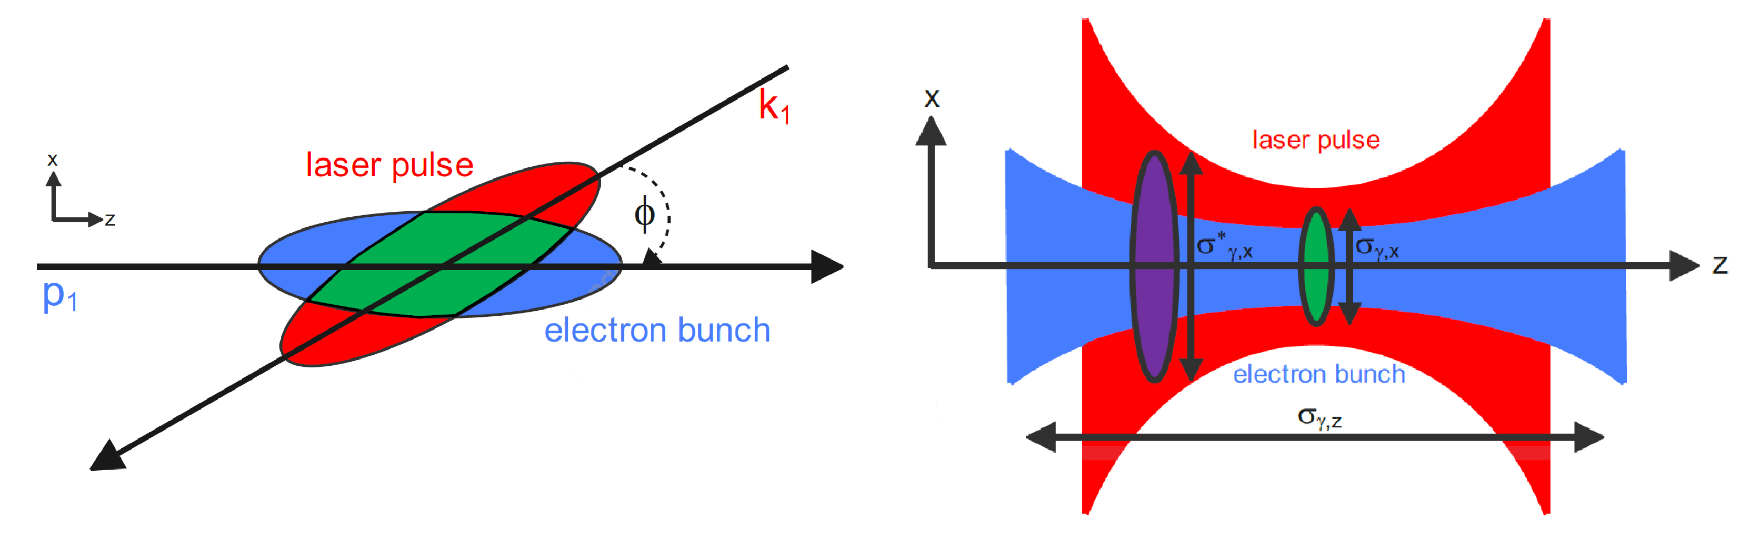
\includegraphics[width=\textwidth]{Figures/Photon_Production_by_Inverse_Compton_Scattering/angular_crossing_hourglass_effect.pdf}
\caption{Left: An electron bunch (blue) interacts with a laser pulse (red) at a crossing angle $\phi$ in the horizontal $x$ plane. The overlap (green) between the electron bunch and laser pulse is reduced due to the crossing angle, leading to a reduction in luminosity. Right: A schematic of the hourglass effect. During an electron bunch--laser pulse interaction both beams diverge longitudinally ($z$ direction) across the interaction source size $\sigma_{\gamma,z}$ (see Section~\ref{sec:source_size_divergence}). Consequently the source size at the waist $\sigma_{\gamma,x}$ (green) is smaller than at other longitudinal positions in the interaction length i.e $\sigma_{\gamma,x}^{*}$ (purple) resulting in a luminosity reduction.}
\label{fig:angular_crossing_hourglass_effect}
\end{figure}

The effect of an angular crossing, which is assumed to be in the horizontal $x$ plane, can be expressed by a reduction factor $R_{AC}$ \cite{suzuki1976general,miyahara2008luminosity}
\begin{equation}
R_{AC} = \frac{\sigma_{x}\cos\phi}{\sqrt{\sigma_{x}^{2}\cos^{2}\phi+\sigma_{z}^{2}\sin^{2}\phi}} = \frac{1}{\sqrt{1+\left(\sigma_{z}^{2}/\sigma_{x}^{2}\right)\tan^{2}\phi}},
\label{eq:angular_crossing_factor}    
\end{equation}
where $\sigma_{z,L} = ct_{pulse}$ with $t_{pulse}$, the laser pulse duration. The luminosity for an angular crossing becomes $\mathcal{L} = R_{AC}\mathcal{L}_{\mathrm{HEAD-ON}}$, therefore the flux in the case of an angular crossing is given by 
\begin{align}
\mathcal{F} &= \sigma R_{AC}\mathcal{L}_{\mathrm{HEAD-ON}}f, \nonumber\\
\mathcal{F} &= \sigma\frac{N_{e}N_{L}f\cos\phi}{2\pi\sigma_{y}\sqrt{\sigma_{x}^{2}\cos^{2}\phi + \sigma_{z}^{2}\sin^{2}\phi}}.
\label{eq:crossing_angle_flux}    
\end{align}
For example, for a Nd:YAG laser ($\lambda = 1064$~\si{\nano\meter}) with a 5~\si{\pico\second} pulse duration and a $\sigma_{L} = 30$~\si{\micro\meter} spot size radius interacting with a 500~\si{\mega\electronvolt} kinetic energy electron bunch with a transverse \textit{rms} spot size of 10~\si{\micro\meter} and a \textit{rms} electron bunch length $\sigma_{e,z} = 0.5$~\si{\milli\meter} interacting at a 5\si{\degree} crossing angle, the angular crossing luminosity factor becomes $R_{AC} = 0.22$ i.e a factor $\sim5$ reduction in luminosity.

The hourglass effect, depicted in Fig.~\ref{fig:angular_crossing_hourglass_effect}, is another deleterious effect on the luminosity of the interaction, where the divergence of two colliding beams is taken into account. As the electron bunch and laser pulse overlap, they diverge and their transverse profiles increase in size which in turn reduces the luminosity. The laser pulse typically diverges quicker than the electron bunch. The reduction factor of the hourglass effect $R_{HG}$ for the head-on case ($\phi = 0$), described by M Furman \cite{furman1991hourglass}, for a beam--beam collision of asymmetric particle beams is altered for the electron bunch--photon pulse collision, where an electron beam divergence term in $t_{x/y}$ is replaced with a photon pulse divergence term, yielding
\begin{equation}
R_{HG} = \frac{1}{\sqrt{\pi}}\int_{-\infty}^{\infty}\frac{\exp\left(-t^{2}\right)}{\sqrt{\left(1+t^{2}/t_{x}^{2}\right)\left(1+t^{2}/t_{y}^{2}\right)}}dt,
\label{eq:furman_hourglass_reduction}    
\end{equation}
where $t$ is the integration variable and the $t_{x/y}$ parameters are given by
\begin{equation}
t_{x/y} = \sqrt{\frac{2\sigma_{x/y}^{2}}{\sigma_{z}^{2}\left(\sigma_{x/y,e}^{2}/\beta_{x/y}^{*2}+\sigma_{L}^{2}/z_{R}^{2}\right)}};
\label{eq:furman_txy_parameters}    
\end{equation}
$\beta_{x/y}^{*}$ are the $\beta$-functions of the electron beam at the interaction point and $z_{R}$ is the Rayleigh range (Eq.~\ref{eq:rayleigh_range}).

An analytical solution to (Eq.~\ref{eq:furman_hourglass_reduction}) can be found for the case of round electron beams ($\sigma_{x,e}=\sigma_{y,e}$) since $t_{x}=t_{y}=t_{RB}$ yielding
\begin{equation}
R_{HG} = \sqrt{\pi}t_{RB}\exp\left(t_{RB}^{2}\right)\left[1-\Phi\left(t_{RB}\right)\right],
\label{eq:furman_hourglass_reduction_analytical}    
\end{equation}
where $1-\Phi\left(t_{RB}\right)$ is the complementary error function of $t_{RB}$. The error function $\Phi$ is defined as
\begin{equation}
\Phi\left(x\right) = \frac{2}{\sqrt{\pi}}\int_{0}^{x}\exp\left(-t^{2}\right)dt,
\label{eq:error_function}    
\end{equation}
where $t$ is the integration variable. Non-round electron bunch transverse profiles must be evaluated using numerical integration of (Eq.~\ref{eq:furman_hourglass_reduction}). For example, for a Nd:YAG laser ($\lambda = 1064$~\si{\nano\meter}) with a 20~\si{\pico\second} pulse duration and a $\sigma_{L} = 30$~\si{\micro\meter} spot size interacting head-on ($\phi=0$) with a 500~\si{\mega\electronvolt} kinetic energy electron bunch with a transverse \textit{rms} spot size of 10~\si{\micro\meter} and \textit{rms} electron bunch length $\sigma_{e,z} = 3$~\si{\milli\meter} yields an hourglass effect luminosity reduction factor becomes $R_{HG} = 0.93$ i.e a 7\% reduction in luminosity.

Miyahara \cite{miyahara2008luminosity} combines the isolated descriptions of the angular crossing by Suzuki \cite{suzuki1976general}, and the hourglass effect by Furman \cite{furman1991hourglass}. The combined angular crossing and hourglass effect reduction factor $R_{ACHG}$ is defined as
\begin{equation}
R_{ACHG} = \int_{-\infty}^{\infty}\frac{H\exp\left(-hZ_{c}^{2}\right)}{\sqrt{\sigma_{x}^{2}+\langle U_{x}^2\rangle Z_{c}^{2}}\sqrt{\sigma_{y}^{2}+\langle U_{y}^{2}\rangle Z_{c}^{2}}}dZ_{c},
\label{eq:miyahara_combined_reduction}    
\end{equation}
where $Z_{c}$ is an integration variable, and the parameters $H$ and $h$ are given by
\begin{align}
H &= \cos\phi\sqrt{\frac{\sigma_{x}^{2}\sigma_{y}^{2}}{\pi\sigma_{z}^{2}}},
\label{eq:miyahara_H_parameter} \\
h &= \frac{\sin^{2}\phi}{\sigma_{x}^{2}+\langle U_{x}^{2}\rangle Z_{c}^{2}}+\frac{\cos^{2}\phi}{\sigma_{z}^{2}};
\label{eq:miyahara_h_parameter}
\end{align}
the divergence term $\langle U_{x/y}^{2}\rangle$ of the electron bunch--laser pulse interaction is
\begin{equation}
\langle U_{x/y}^{2}\rangle = \frac{\left(\sigma_{x/y,e}^{2}/\beta_{x/y}^{*2}\right)+\left(\sigma_{L}^{2}/z_{R}^{2}\right)}{2}.    
\end{equation}
The combined reduction factor $R_{ACHG}$ must be evaluated numerically as no analytical solutions exist. With short picosecond-scale laser pulses and electron bunches the hourglass effect contribution can be minimal when there is a crossing angle between the electron bunch and laser pulse. For example, for a Nd:YAG laser ($\lambda = 1064$~\si{\nano\meter}) with a 5~\si{\pico\second} pulse duration and a $\sigma_{L} = 30$~\si{\micro\meter} spot size interacting at a 5\si{\degree} crossing angle with a 500~\si{\mega\electronvolt} kinetic energy electron bunch with a transverse \textit{rms} spot size of 10~\si{\micro\meter} and a \textit{rms} electron bunch length $\sigma_{e,z} = 0.5$~\si{\milli\meter} the angular crossing luminosity factor becomes $R_{ACHG} = 0.22$. For the identical situation $R_{AC} = 0.22$, so the hourglass effect is negligible, because the crossing angle reduces the interaction time and is consequently the dominant factor in geometric luminosity reduction.

\subsection{Geometric Luminosity Reduction Benchmarking}

The geometric luminosity reduction calculation (Eq.~\ref{eq:miyahara_combined_reduction}) has been extensively benchmarked and the results of Miyahara's paper \cite{miyahara2008luminosity} have been replicated here. Fig.~\ref{fig:miyahara_benchmarking} shows the replication of Fig.~6 of Miyahara's work \cite{miyahara2008luminosity} (based on the Table~1 parameters) using \textsc{Mathematica} with trapezium rule integration to numerically evaluate (Eq.~\ref{eq:miyahara_combined_reduction}). Inspection of the two plots in Fig.~\ref{fig:miyahara_benchmarking} shows that they are the same. Therefore, (Eq.~\ref{eq:miyahara_combined_reduction}) is a reliable method to account for the angular crossing and hourglass effect luminosity reduction factors. 
\begin{figure}[!h]
\centering
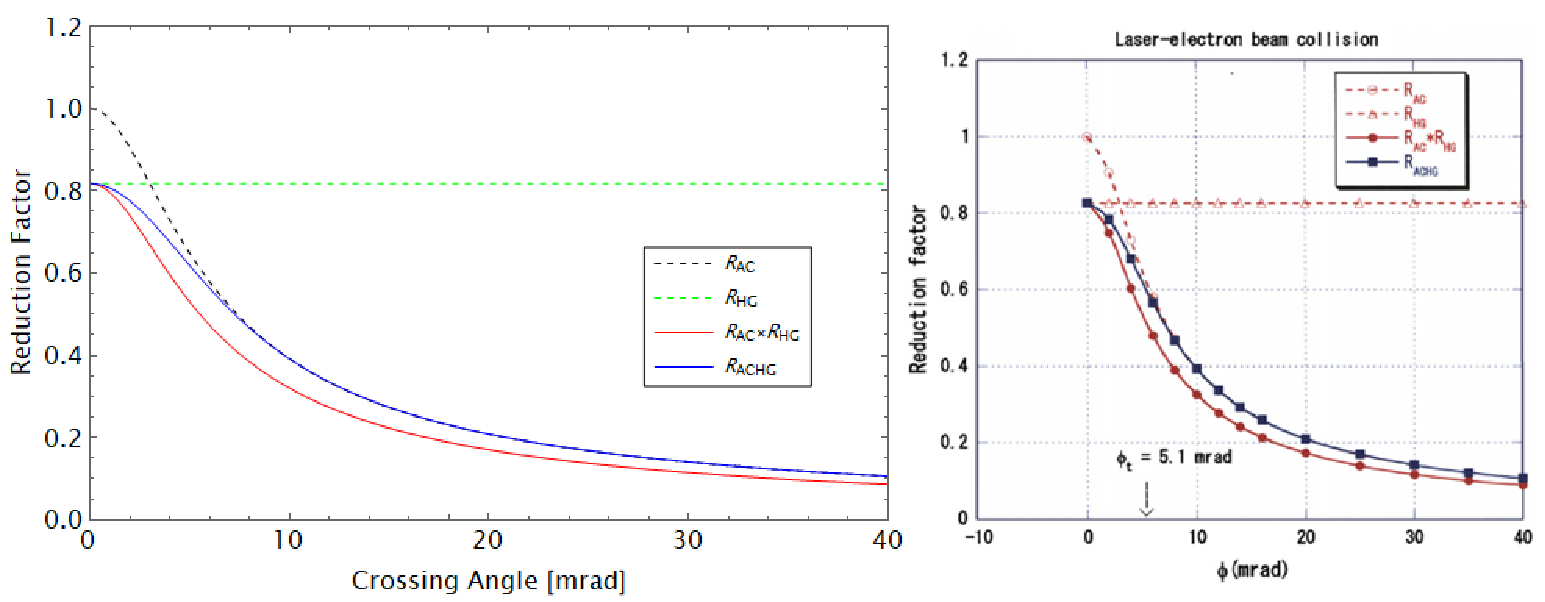
\includegraphics[width=\textwidth]{Figures/Photon_Production_by_Inverse_Compton_Scattering/miyahara_benchmarking.pdf}
\caption{Benchmarking of (Eq.~\ref{eq:miyahara_combined_reduction}) with the results of Miyahara \cite{miyahara2008luminosity}, for the Table~1 parameters and results shown in Fig.~6 of the paper. Other equations are also benchmarked such as (Eq.~\ref{eq:angular_crossing_factor}) and (Eq.~\ref{eq:furman_hourglass_reduction_analytical}). Left: Replication plot showing the angular crossing reduction $R_{AC}$ (black), hourglass reduction $R_{HG}$ (green), crudely combined reduction $R_{AC}\times R_{HG}$ (red) and combined reduction $R_{ACHG}$ (blue). Right: Reproduction of Fig.~6 of Miyahara \cite{miyahara2008luminosity} showing the angular crossing $R_{AC}$ (red dashed circles), hourglass effect $R_{HG}$ (red dashed triangles), crude combination $R_{AC}\timesR_{HG}$ (red solid) and combined $R_{ACHG}$ (black) reduction factors.}
\label{fig:miyahara_benchmarking}
\end{figure}

The flux in the case of an angular collision with non-negligible divergence of electron bunches and laser pulses (hourglass effect) is given by
\begin{equation}
\mathcal{F} = \sigma f R_{ACHG}\mathcal{L}_{\mathrm{HEAD-ON}}.
\label{eq:flux_angular_crossing_hourglass}
\end{equation}
All subsequent equations, unless explicitly stated, use (Eq.~\ref{eq:flux_angular_crossing_hourglass}) to account for the geometric luminosity reduction of an ICS source. The luminosity of this result is given by $\mathcal{L} = R_{ACHG}\mathcal{L}_{\mathrm{HEAD-ON}}$, mirroring the form of the luminosity for the isolated angular crossing and hourglass effect.

Naively, one would expect the luminosity to also be appropriately modelled by $\mathcal{L} = R_{AC}R_{HG}\mathcal{L}_{\mathrm{HEAD-ON}}$, however this is incorrect as a moderate crossing angle $\phi$ will shorten the interaction time between the laser pulse and electron beam such that the interaction length is of an order at which the electron bunch and laser pulse minimally diverge and the hourglass effect is negligible. Effectively, as shown by the example calculations, a moderate crossing angle suppresses the hourglass effect.   

\section{Source Size and Divergence}
\label{sec:source_size_divergence}

The derivation of luminosity and flux in Section~\ref{sec:luminosity_and_flux} has assumed that all emission of radiation in the ICS interaction is from a point source at the centre of the interaction. However, the electron--photon interaction occurs in a finite spatial volume and the transverse size of this spatial volume is here named the source size. The source transverse density (electrons per transverse area) is given by the transverse electron bunch electron density $n_{e}\left(x,y\right)$ and transverse laser pulse photon density $n_{L}\left(x,y\right)$ \cite{krafft2020personal}
\begin{equation}
n_{s}\left(x,y\right) = n_{e}\left(x,y\right) n_{L}\left(x,y\right),
\label{eq:transverse_source_approx}    
\end{equation}
Modification of the Gaussian intensity distributions of the electron bunch (Eq.~\ref{eq:electron_gaussian_intensity_distribution}) and laser pulse (Eq.~\ref{eq:laser_gaussian_intensity_distribution}) results in the transverse densities of the photon pulse and electron bunch
\begin{align}
n_{e}\left(x,y\right) &= \frac{N_{e}}{2\pi\sigma_{e}^{2}}\exp\left(-\frac{x^{2}+y^{2}}{2\sigma_{e}^{2}}\right), 
\label{eq:transverse_electron_bunch_density}\\ 
n_{L}\left(x,y\right) &= \frac{N_{L}}{2\pi\sigma_{L}^{2}}\exp\left(-\frac{x^{2}+y^{2}}{2\sigma_{L}^{2}}\right).
\label{eq:trasverse_photon_pulse_density}
\end{align}
The transverse density of the source (Eq.~\ref{eq:transverse_source_approx}) can be expanded through substitution of the transverse electron (Eq.~\ref{eq:transverse_electron_bunch_density}) and photon (Eq.~\ref{eq:trasverse_photon_pulse_density}) densities 
\begin{align}
n_{s}\left(x,y\right) = \frac{N_{e}}{2\pi\sigma_{e}^{2}}\exp\left(-\frac{x^{2}+y^{2}}{2\sigma_{e}^{2}}\right)\frac{N_{L}}{2\pi\sigma_{L}^{2}}\exp\left(-\frac{x^{2}+y^{2}}{2\sigma_{L}^{2}}\right), \nonumber \\
n_{s}\left(x,y\right) = \frac{N_{e}N_{L}}{2\pi\sigma_{e}^{2}\sigma_{L}^{2}}\exp\left[-\frac{\left(x^{2}+y^{2}\right)\left(\sigma_{e}^{2}+\sigma_{L}^{2}\right)}{\sigma_{e}^{2}\sigma_{L}^{2}}\right], \nonumber \\
n_{s}\left(x,y\right) = \frac{1}{2\pi\left(\sigma_{e}^{2}+\sigma_{L}^{2}\right)}\frac{1}{2\pi\sigma_{\gamma}^{2}}\exp\left(-\frac{x^{2}+y^{2}}{2\sigma_{\gamma}^{2}}\right),
\label{eq:expanded_transverse_source_density}    
\end{align}
where the transverse \textit{rms} source size of an inverse Compton scattering electron bunch--laser pulse interaction is consequently defined as
\begin{equation}
\sigma_{\gamma,x/y} = \frac{\sigma_{e,x/y}\sigma_{L}}{\sqrt{\sigma_{e,x/y}^{2}+\sigma_{L}^{2}}},
\label{eq:source_size}
\end{equation}
where $\sigma_{e,x/y}$ is the \textit{rms} transverse electron bunch spot size in each plane and $\sigma_{L}$ is the \textit{rms} transverse laser pulse spot size. A similar derivation to (Eq.~\ref{eq:expanded_transverse_source_density}) can be made for the longitudinal domain, therefore the longitudinal \textit{rms} source size is given by
\begin{equation}
\sigma_{\gamma,z} = \frac{\sigma_{e,z}\left(ct_{\mathrm{pulse}}\right)}{\sqrt{\sigma_{e,z}^{2}+\left(ct_{\mathrm{pulse}}\right)^{2}}},
\label{eq:longitudinal_source_size}
\end{equation}
where $\sigma_{e,z}$ is the \textit{rms} electron bunch length and $t_{\mathrm{pulse}}$ is the \textit{rms} photon pulse duration. 

Similarly to the \textit{rms} transverse source size, the \textit{rms} source angular divergence of an ICS interaction is
\begin{equation}
\sigma_{\gamma,x/y}' = \frac{\sigma_{e,x/y}'\sigma_{L}'}{\sqrt{\sigma_{e,x/y}'^{~2}+\sigma_{L}'^{~2}}},
\label{eq:source_divergence}
\end{equation}
where $\sigma_{e,x/y}' = \sqrt{\epsilon_{x}/\beta_{x}^{*}}$ is the \textit{rms} transverse electron bunch angular divergence for a non-diffraction limited beam and $\sigma_{L} = \sqrt{\lambda/4\pi}$ is the \textit{rms} transverse laser pulse angular divergence.

A non-zero transverse source size (Eq.~\ref{eq:source_size}) suggests that photon emission from the ICS interaction can occur from any transverse position within the source. Whilst the emission of radiation would occur mostly frequently in the centre of the bunch emission would also be possible from the edges of the source. A non-zero source size with possible emission from a finite transverse (Eq.~\ref{eq:source_size}) and longitudinal (Eq.~\ref{eq:longitudinal_source_size}) source would appear to invalidate the point source approximation used in Section~\ref{sec:luminosity_and_flux}. However, the point source approximation holds if the scattered photon distribution is sampled a large distance from the source relative to the source size i.e $d \gg \sigma_{\gamma,z}$, where $d$ is the source to collimator/detector distance. When $d \gg \sigma_{\gamma,z}$ holds this is termed far-field collimation, as valid for our discussion of collimation in ICS sources in Section~\ref{sec:analytical_collimated_flux}. Far-field collimation can be stated analogously in the transverse plane as $a \gg \sigma_{\gamma,x/y}$, where $a$ is the transverse size of a collimator or detector aperture downstream of the interaction. The far-field collimation condition is obeyed by all ICS sources designed within this work.  

\section{Bandwidth}
\label{sec:bandwidth}

\subsection{Bandwidth of an ICS Source}

The bandwidth -- the \textit{rms} energy spread of the scattered photons -- of an ICS source as derived by Ranjan et al \cite{ranjan2018simulation} is given by
\begin{equation}
\frac{\Delta E_{\gamma}}{E_{\gamma}} = \sqrt{\left(\frac{\sigma_{\theta}}{E_{\theta}}\right)^{2}+\left(\frac{\sigma_{e}}{E_{e}}\right)^{2}+\left(\frac{\sigma_{L}}{E_{L}}\right)^{2}+\left(\frac{\sigma_{\epsilon}}{E_{\epsilon}}\right)^{2}},
\label{eq:RMS_bandwidth}    
\end{equation}
where $\sigma_{\theta}/E_{\theta}$ is a collimation term, $\sigma_{e}/E_{e}$ is an electron beam energy spread term, $\sigma_{L}/E_{L}$ is a laser pulse energy spread term and $\sigma_{\epsilon}/E_{\epsilon}$ is an emittance term. The Ranjan et al bandwidth (Eq.~\ref{eq:RMS_bandwidth}) is valid for the recoil corrected ($X\sim 1$) non-linear regime ($a_{0}\ll 1$) and the terms of the bandwidth are given by
\begin{align}
\frac{\sigma_{\theta}}{E_{\theta}} &= \frac{1}{\sqrt{12}}\frac{\Psi^{2}}{1+X+\Psi^{2}/2},
\label{eq:collimation_term} \\
\frac{\sigma_{e}}{E_{e}} &= \frac{2+X}{1+X+\Psi^{2}}\frac{\Delta E_{e}}{E_{e}},
\label{eq:beam_energy_spread_term} \\
\frac{\sigma_{L}}{E_{L}} &= \frac{1+\Psi^{2}}{1+X+\Psi^{2}}\frac{\Delta E_{L}}{E_{L}},
\label{eq:laser_energy_spread_term} \\
\frac{\sigma_{\epsilon}}{E_{\epsilon}} &= \frac{\sqrt{2}\gamma^{2}}{1+X}\sqrt{\frac{\epsilon_{x}^{2}}{\beta_{x}^{*2}}+\frac{\epsilon_{y}^{2}}{\beta_{y}^{*2}}}
\label{eq:emittance_term}
\end{align}
where $\Psi = \gamma\theta$ is the acceptance angle, $\epsilon_{x/y}$ is the emittance in the $x$ or $y$ direction, $\beta_{x/y}^{*}$ are the $\beta$ functions at the IP in both directions, $\Delta E_{e}/E_{e}$ is the \textit{rms} relative energy spread of the electron bunch and $\Delta E_{L}/E_{L}$ is the \textit{rms} spectral bandwidth of the laser pulse.

The electron bunch energy spread term (Eq.~\ref{eq:beam_energy_spread_term}) and laser pulse energy spread term (Eq.~\ref{eq:}) describe how the energy spreads of the electron bunch and spectral bandwidth of the laser pulse transform to the energy spread of the scattered radiation. Off-momentum electrons in the electron beam are interacted with the laser and are scattered to produce higher or lower energy scattered photons, the analogous situation happens with incident photons of variable energy. The collimation term (Eq.~\ref{eq:collimation_term}) arises because photons emitted with different scattering angle have different energies, so for a particular maximum scattering angle (collimation angle) there is an associated energy spread in the scattered radiation. Emittance of the electron beam corresponds to an associated energy spread in the scattered photons because electrons can interact off-axis in the collision, which means they can pass through the collimator with a larger scattering angle and lower energy. Ranjan et al \cite{ranjan2018simulation} present a full derivation of the emittance broadening of the scattered photon energy.  The effect of off-axis electrons is encapsulated in the emittance term (Eq.~\ref{eq:emittance_term}). 

Conversion of the \textit{rms} bandwidth to the full width half maximum (FWHM) bandwidth is trivial and is given by 
\begin{equation}
\left(\frac{\Delta E_{\gamma}}{E_{\gamma}}\right)_{\mathrm{FWHM}} = 2\sqrt{2\ln{2}}\left(\frac{\Delta E_{\gamma}}{E_{\gamma}}\right)_{rms} \approx 2.355\left(\frac{\Delta E_{\gamma}}{E_{\gamma}}\right)_{rms}.
\label{eq:FWHM_bandwidth}
\end{equation}

\subsection{Other Bandwidth Formulations}

Other formulations of the \textit{rms} bandwidth exist such as the formulation derived by Petrillo et al \cite{petrillo2012photon,akagi2016narrow}:
\begin{equation}
\frac{\Delta E_{\gamma}}{E_{\gamma}} = \sqrt{\Psi^{4}+4\left(\frac{\Delta E_{e}}{E_{e}}\right)^{2}+\left(\frac{\epsilon_{n}}{\sigma_{e}}\right)^{4}+\left(\frac{\Delta\nu}{\nu}\right)^{2}+\left(\frac{M^{2}\lambda}{4\pi\sigma_{L}}\right)^{4}},
\label{eq:akagi_bandwidth}    
\end{equation}
where $\epsilon_{n}=\epsilon_{n,x}=\epsilon_{n,y}$ is the round beam normalised transverse emittance, $\sigma_{e}$ is the round beam electron bunch spot size, $\Delta\nu/\nu$ is the spectral bandwidth of the laser pulse defined in terms of the laser pulse frequency $\nu$ and $M^{2}$ is the quality factor of the laser pulse ($M^{2} = 1$ for a perfectly Gaussian laser pulse). In comparison to (Eq.~\ref{eq:RMS_bandwidth}), the formulation used by Akagi et al \cite{akagi2016narrow} is simplistic in the treatment of the emittance term $\left(\epsilon_{n}/\sigma_{e}\right)^{4}$, by solely accounting for the round beam divergence, and the collimation term $\Psi^{4}$ where the recoil dependence is neglected. The Petrillo et al bandwidth is consequently only valid in the round beam case ($\epsilon_{n,x} = \epsilon_{n,y} = \epsilon_{n}$). Recoil of the electron bunch has also not been accounted for in any term, so the Petrillo et al bandwidth is only relevant in the Thomson regime ($X \ll 1$) and angular variation is only accounted for in the collimation term not, as in (Eq.~\ref{eq:RMS_bandwidth}), for the electron bunch $4\left(\Delta E_{e}/E_{e}\right)^{2}$ and laser pulse $\left(\Delta\nu/\nu\right)^{2}$ energy spread terms. Unlike in (Eq.~\ref{eq:RMS_bandwidth}), a laser pulse quality term $\left(M^{2}\lambda/4\pi\sigma_{L}\right)^{4}$ is imposed but this term is generally negligible. For example, for a Gaussian ($M^{2}=1$) Nd:YAG laser ($\lambda = 1064$~\si{\nano\meter}) pulse focused to a typical small laser pulse \textit{rms} spot size of 30~\si{\micro\meter} this term makes a $7.97\times 10^{-6}$ contribution to the \textit{rms} bandwidth hence it is neglected by Ranjan et al \cite{ranjan2018simulation} in the selected \textit{rms} bandwidth (Eq.~\ref{eq:RMS_bandwidth}).   

Another possible formulation has been suggested by Curatolo et al \cite{curatolo2017analytical}, which updates (Eq.~\ref{eq:akagi_bandwidth}) to be
\begin{multline}
\frac{\Delta E_{\gamma}}{E_{\gamma}} = \left\{\left[\frac{\Psi^{2}}{\sqrt{12}\left(1+\Psi^{2}\right)}+\frac{\bar{P}^{2}}{1+\sqrt{12}\bar{P}^{2}}\right]^{2}+\left[\left(\frac{2+X}{1+X}\right)\frac{\Delta E_{e}}{E_{e}}\right]^{2}+\left(\frac{1}{1+X}\frac{\Delta E_{L}}{E_{L}}\right)^{2} \right.\\\left. +\left(\frac{M^{2}\lambda}{4\pi\sigma_{L}}\right)^{4}+\left(\frac{a_{0}^{2}/3}{1+a_{0}^{2}/2}\right)^{2}\right\}^{1/2}
\label{eq:curatolo_bandwidth}    
\end{multline}
where 
\begin{equation}
\bar{P} = \frac{\sqrt{2}\epsilon_{n}}{\sigma_{e}\sqrt{1+X}},
\label{eq:curatolo_p_bar}    
\end{equation}
is the \textit{rms} normalised transverse momentum of the electron bunch. The bandwidth formulation by Curatolo et al assumes a round transverse profile of the electron bunch as in (Eq.~\ref{eq:akagi_bandwidth}), and also includes an identical beam quality term, which is previously shown to be generally negligible. Recoil correction is included in (Eq.~\ref{eq:curatolo_bandwidth}) but angular variation is only included in the collimation term, as the acceptance angle is present in no other term. A non-linear ponderomotive broadening term $\left(\frac{a_{0}^{2}/3}{1+a_{0}^{2}/2}\right)^{2}$ is introduced in (Eq.~\ref{eq:curatolo_bandwidth}), which is advantageous over the bandwidth by Ranjan et al \cite{ranjan2018simulation} where non-linear effects are not accounted for. 

The bandwidth by Curatolo et al \cite{curatolo2017analytical} also includes covariance of the emittance and collimation terms for predicting the bandwidth of skewed non-Gaussian scattered photon spectra \cite{ranjan2018simulation} produced when the ICS interaction is not between a Gaussian electron bunch and laser pulse. However, skewed non-Gaussian spectral effects can also be accounted for using a modified version of Ranjan et al's bandwidth
\begin{equation}
\frac{\Delta E_{\gamma}}{E_{\gamma}} = \sqrt{\left[\left(\frac{\sigma_{\theta}}{E_{\theta}}\right)+\left(\frac{\sigma_{\epsilon}}{E_{\epsilon}}\right)\right]^{2}+\left(\frac{\sigma_{e}}{E_{e}}\right)^{2}+\left(\frac{\sigma_{L}}{E_{L}}\right)^{2}},
\label{eq:covariant_RMS_bandwidth}    
\end{equation}
where the emittance and collimation terms are covariant. The covariant form (Eq.~\ref{eq:covariant_RMS_bandwidth}), whilst more general, is not utilised in this work because there is a focus on Gaussian electron bunches and laser pulses, and (Eq.~\ref{eq:RMS_bandwidth}) produces the same result as (Eq.~\ref{eq:covariant_RMS_bandwidth}) for Gaussian ICS spectra. All optimisation methods in Chapter~\ref{Optimisation_and_Characterisation_of_Inverse_Compton Scattering_Spectra} can be utilised with the covariant form, however as standard (Eq.~\ref{eq:RMS_bandwidth}) is used. 

Therefore, (Eq.~\ref{eq:RMS_bandwidth}) was selected as this is both recoil--corrected and accounts for angular variation in each bandwidth term; it is valid in the linear ($a_{0}\ll 1$) region of interest and most importantly, properly accounts for non-round electron bunch transverse profiles by allowing for asymmetric emittance ($\epsilon_{n,x}\neq\epsilon_{n,y}$).  As shown in Fig.~1 of Ranjan et al \cite{ranjan2018simulation} (reproduced in Fig.~\ref{fig:curatolo_ranjan_disagreement}), there is also an apparent discrepancy in how the collimation angle, via the acceptance angle $\psi = \gamma\theta$, is accounted for in the Curatolo et al equation (Eq.~\ref{eq:curatolo_bandwidth}). Whilst the semi-analytical spectrum code \textsc{ICCS3D} \cite{krafft2016laser,ranjan2018simulation} (explained further in Chapter~\ref{Optimisation_and_Characterisation_of_Inverse_Compton Scattering_Spectra}) and (Eq.~\ref{eq:RMS_bandwidth}) show good agreement, (Eq.~\ref{eq:curatolo_bandwidth}) shows a systematic difference from these simulations. The combination of these factors provided the motivation for selecting (Eq.~\ref{eq:RMS_bandwidth}) as the \textit{rms} bandwidth formulation.
\begin{figure}[!h]
\centering
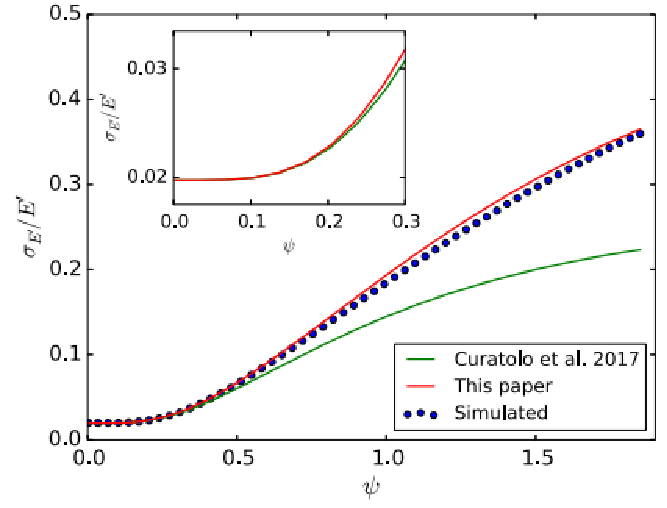
\includegraphics[width=0.7\textwidth]{Figures/Photon_Production_by_Inverse_Compton_Scattering/ranjan_curatolo_disagreement.pdf}
\caption{Reproduction of Fig.~1 of Ranjan et al \cite{ranjan2018simulation}. \textit{Rms} bandwidth of an ICS source as a function of acceptance angle, using the case $A_{a}$ parameters by Ranjan et al \cite{ranjan2018simulation}, for (Eq.~\ref{eq:RMS_bandwidth}) (red, Ranjan et al \cite{ranjan2018simulation}) and (Eq.~\ref{eq:curatolo_bandwidth}) (green, Curatolo et al \cite{curatolo2017analytical}) and the \textsc{ICCS3D} simulated spectrum bandwidths (black points, Ranjan et al \cite{ranjan2018simulation}). }
\label{fig:curatolo_ranjan_disagreement}
\end{figure}

However, there are some downsides to the Ranjan et al formulation (Eq.~\ref{eq:RMS_bandwidth}), as this is incapable of calculating the bandwidth for a non-linear ($a_{0}\sim 1$) ICS source. Circular collimation is also assumed implicitly by the inclusion of a single acceptance angle term $\Psi$, as in the case of a rectangular collimator the maximum collimation angle would vary in each plane. However, the bandwidth in (Eq.~\ref{eq:RMS_bandwidth}) has been extended to rectangular collimation by Hajima \cite{hajima2021bandwidth}, though the ICS sources within this thesis only employ circular collimation so Ranjan et al \cite{ranjan2018simulation} (Eq.~\ref{eq:RMS_bandwidth}) is used. 

\section{Spectral Density}

The spectral density of an ICS source is a measure of the energy density of the produced photon spectrum; a higher spectral density for the same scattered photon energy source means more photons are produced. The spectral density of an inverse Compton scattering source, for the full scattered photon spectrum, is given by
\begin{equation}
\mathcal{S} = \frac{\mathcal{F}}{E_{\gamma}^{\mathrm{MAX}}},
\label{eq:spectral_density}    
\end{equation}
where $\mathcal{F}$ is the total flux of the ICS source given by (Eq.~\ref{eq:flux_angular_crossing_hourglass}) and $E_{\gamma}^{\mathrm{MAX}}$ is the maximum scattered photon energy, also known as the Compton edge energy (Eq.~\ref{eq:compton_edge_energy}), when the incident photon is backscattered ($\theta=0$).

The spectral density can also be measured around the Compton edge energy for a particular bandwidth, for example by replacing the total flux $\mathcal{F}$ with the FWHM flux in a 0.1\% bandwidth $\mathcal{F_{\mathrm{0.1\%}}}$ (Eq.~\ref{eq:flux_0.1_bandwidth}). The spectral density around the Compton edge (Eq.~\ref{eq:compton_edge_energy}) in a 0.1\% \textit{FWHM} bandwidth is therefore
\begin{equation}
\mathcal{S}_{\mathrm{0.1\%}} = \frac{\mathcal{F_{\mathrm{0.1\%}}}}{E_{\gamma}^{\mathrm{MAX}}}.
\label{eq:spectral_density_0.1}    
\end{equation}
Framed in terms of a particular bandwidth, the spectral density becomes an important performance parameter of a narrowband ICS source. If an ICS source has a higher spectral density within a particular bandwidth than another source then this source produces a higher flux of narrowband radiation. Utilising spectral density comparisons within a particular bandwidth around the Compton edge is a more appropriate comparative measure of ICS source performance because a user can understand the energy density of photons available to a particular experiment from an ICS source.   

\section{Peak and Average Brilliance}
\label{sec:peak_average_brilliance}

Brilliance, sometimes termed brightness, is a quantity originally used by Courant and Snyder \cite{courant1958theory} to quantify the 6D phase space density of particle beams. The concept of brilliance was adopted to characterize radiation beams produced from accelerator driven light sources, such as bending magnet or wiggler synchrotron radiation sources and undulators \cite{kim1989characteristics}, where the brilliance is defined as the flux of photons into a particular bandwidth (usually 0.1\% FWHM) per unit phase space area. Here, brilliance is used to describe photon beams and brightness to describe the similar concept in electron beams (Eq.~\ref{eq:electron_brightness}). The brilliance performance parameter is readily applied to synchrotron radiation sources, free electron lasers \cite{krinsky1983undulators,kim1987brightness} and has been extended to ICS sources \cite{hartemann2005high,krafft2010compton}.

Brilliance is an important measure for synchrotron radiation sources because these typically use a monochromator to achieve a small bandwidth. Monochromation is achieved by taking advantage of the photon energy dependency of the Bragg condition (Eq.~\ref{eq:Bragg_condition}) and collecting photons (from the radiation source) that are scattered into a particular diffraction angle, which are of small energy spread (bandwidth). However, monochromators can only function when the photons incident on it (from the radiation source) are from a similar angle and position. Therefore, a small spot size and divergence of the emitted radiation is required at the monochromator for effective selection of a small bandwidth. As brilliance measures the flux of photons as a function of phase space -- the size and divergence of the emitted radiation -- a high brilliance source translates to a high flux of monochromatic photon post monochromator. Hence, brilliance is used to characterise synchrotron radiation source. For an ICS source brilliance is a less important measure because, as shown in Section~\ref{sec:derivation_of_the_scattered_photon_energy}, emitted photons from an ICS source do not require a monochromator. 

Average brilliance is time averaged, summing the contribution of all electron bunch--laser pulse interactions of the source, thereby accounting for the repetition rate of the interactions. Peak brilliance is calculated for a single bunch--pulse interaction subject to the pulse duration of the emitted radiation. Both peak and average brilliance have advantages for different users; large peak brilliance is useful for analysing processes which occur on a timescale shorter than the timescale for two radiation pulses to be emitted and in making destructive measurements -- similar to the utility of x-ray FELs \cite{emma2010first}. Whereas average brilliance excels in improving data acquisition rates in processes with small cross sections, such as nuclear resonance fluorescence studies \cite{angell2015demonstration}. Linac driven ICS sources typically are designed to be single-shot, high peak brilliance sources whereas storage ring and recirculated electron beam based ICS sources take advantage of high repetition rates to be high average brilliance sources. Theoretically, ERLs with linac-quality re-circulated electron beams could provide high peak and average brilliance simultaneously.   

\subsection{Average Brilliance}

ICS sources can be viewed as analogous to undulator radiation -- a `laser undulator' system. Hence, the average brilliance of an ICS source is adapted from that of an undulator. The average brilliance of an undulator source assuming a Gaussian electron bunch and planar undulator field \cite{chao2013handbook} is given by 
\begin{equation}
\mathcal{B}_{U} = \frac{\Phi_{n}}{4\pi^{2}\Sigma_{x}\Sigma_{y}\Sigma_{x}'\Sigma_{y}'}
\label{eq:undulator_brightness}    
\end{equation}
where $\Phi_{n}$ is the total flux of the $n$th undulator harmonic generated into a central cone of 0.1\% FWHM bandwidth, $\Sigma_{x/y} = \sqrt{\sigma_{x/y}^{2}+\sigma_{R}^{2}}$ are the effective source sizes in each plane (with $\sigma_{x/y}$ the \textit{rms} source size of the electron beam and $\sigma_{R}$ the diffraction-limited source size of a single electron emission \cite{kim1987brightness}), and $\Sigma_{x/y}' = \sqrt{\sigma_{x}'^{2}+\sigma_{R}'^{2}}$ the source size divergences (with $\sigma_{x}'$ the \textit{rms} divergence of the electron beam and $\sigma_{R}'$ the \textit{rms} angular divergence of the single electron emission \cite{krinsky1983undulators}). 

The average brilliance for an inverse Compton scattering source is defined as the average flux per unit phase space area of the interaction per 0.1\% FWHM bandwidth. The ICS average brilliance is modified from the undulator brilliance (Eq.~\ref{eq:undulator_brightness}) through replacement of the single electron emission field for the electric field of a Gaussian laser pulse \cite{krafft2010compton,deitrick2018high}
\begin{equation}
\mathcal{B}_{\mathrm{avg}} = \frac{\mathcal{F}_{0.1\%}}{4\pi^{2}\sigma_{\gamma,x}\sigma_{\gamma,x}'\sigma_{\gamma,y}\sigma_{\gamma,y}'},
\label{eq:average_brilliance}
\end{equation}
where $\mathcal{F}_{0.1\%}$ is the flux in a 0.1\% FWHM bandwidth (Eq.~\ref{eq:flux_0.1_bandwidth}) using the modified form of the flux for geometric luminosity reduction (Eq.~\ref{eq:flux_angular_crossing_hourglass}), $\sigma_{\gamma,x/y}$ are the source sizes in each plane (Eq.~\ref{eq:source_size}) and $\sigma_{\gamma,x/y}'$ are the source angular divergences (Eq.~\ref{eq:source_divergence}) in each plane. Assuming a non-diffraction-limited electron bunch and that $\sigma_{e,x/y}' > \sigma_{L}'$, the brilliance can be calculated as
\begin{equation}
\mathcal{B}_{\mathrm{avg}} = \frac{\mathcal{F}_{0.1\%}}{4\pi^{2}\sigma_{\gamma,x}\sqrt{\epsilon_{x}/\beta_{x}^{*}}\sigma_{\gamma,y}\sqrt{\epsilon_{y}\beta_{y}^{*}}}.
\label{eq:average_brilliance_nondiffraction}    
\end{equation}
Simplifying (Eq.~\ref{eq:average_brilliance_nondiffraction}) further, by noting that for a compact ICS source the electron bunch transverse profile size is typically larger than the laser spot size ($\sigma_{e,x/y}\gg\sigma_{L}$) i.e $\sigma_{\gamma,x/y} \approx \sqrt{\epsilon_{x/y}\beta_{x/y}^{*}}$, the average brilliance becomes
\begin{equation}
\mathcal{B}_{\mathrm{avg}} \approx \frac{\gamma^{2}\mathcal{F}_{0.1\%}}{4\pi^{2}\epsilon_{n,x}\epsilon_{n,y}}.
\label{eq:average_brilliance_compact}    
\end{equation}
Therefore the average brilliance is $\mathcal{B}\propto 1/\gamma^{2}$ because the scattered photon beam is projected into a $1/\gamma$ cone in each plane and the angular dependence is incorporated into the scattered photon beam phase space.   

However, an assumption of $\sigma_{L}<\sigma_{e}$ is often incorrect for the source designs presented in this thesis and Section~\ref{sec:transverse_profile_matching} makes a case for narrowband ICS sources with $\sigma_{L}>\sigma_{e}$; therefore (Eq.~\ref{eq:average_brilliance_compact}) is not used here. The angular divergence of the electron bunch is also not typically larger than the angular divergence of the laser pulse in a narrowband ICS source. For example, using the derivations of Section~\ref{sec:source_size_divergence}, a Nd:YAG laser ($\lambda = 1064$~\si{\nano\meter}) interacting with a $E_{e} = 500$~\si{\mega\electronvolt} kinetic energy electron bunch with a 0.5~\si{\mill\meter}--\si{\milli\radian} normalised emittance in each plane at a focus of $\sigma_{e} = 10$~\si{\centi\meter} in each plane has an electron bunch angular divergence of $\sigma_{e}' = 7.14\times10^{-5}$~\si{\radian} and a laser pulse angular divergence of $\sigma_{L}' = 2.91\times 10^{-4}$~\si{\radian}. Clearly, the effect of the laser pulse angular divergence in (Eq.~\ref{eq:average_brilliance}) can not be neglected in all cases so (Eq.~\ref{eq:average_brilliance}) is favoured over (Eq.~\ref{eq:average_brilliance_nondiffraction}), where the laser pulse angular divergence is neglected.  

\subsection{Peak Brilliance}
The peak brilliance -- the brilliance of a single ICS interaction subject to the duration of the scattered photon pulse -- can also be defined for an ICS source, as for a FEL. Hartemann and Brown \cite{hartemann2005high} derive the peak brilliance to be given by
\begin{multline}
\mathcal{B}_{\mathrm{pk}} = \frac{4\times 10^{-15}}{\pi^{2}}\frac{\gamma}{\epsilon_{n}^{2}}\frac{N_{e}N_{L}}{t_{\mathrm{bunch}}}\frac{r_{e}^{2}}{4\sigma_{L}^{2}}\exp\left\{\frac{\chi-1}{2\chi\Delta u_{\perp}^{2}}\left[2+\frac{\delta\omega^{2}+\delta\gamma^{2}\chi^{2}}{2\chi\left(\chi-1\right)\Deltau_{\perp}^{2}}\right]\right\} \\ \left[1-\Phi\left\{\frac{\chi-1}{\sqrt{\delta\omega^{2}+\delta\gamma^{2}\chi^{2}}}\left[1+\frac{\delta\omega^{2}+\delta\gamma^{2}\chi^{2}}{2\cji\left(\chi-1\right)\Delta u_{\perp}^{2}}\right]\right\}\right]\left\{\frac{\eta e^{1/\mu^{2}\left[\Phi\left(1/\eta\right)-1\right]-\mu e^{1/\eta^{2}}\left[\Phi\left(1/\mu\right)-1\right]}}{\mu^{2}-\eta^{2}}\right\},
\label{eq:hartemann_peak_brilliance}    
\end{multline}
where $\chi = E_{\gamma}/4\gamma^{2}E_{L}$ is the normalised Doppler up-shifted frequency (the ratio of the scattered photon energy and Compton edge energy (Eq.~\ref{eq:compton_edge_energy})) and $\Delta u_{\perp} \approx \epsilon_{n}/\sigma_{e}$ is the approximate transverse spread in electron velocity -- assuming the transverse velocity of the electron beam is small before the interaction. The relative spectral bandwidth of the laser pulse is given by $\delta\omega = 2\Delta E_{L}/E_{L}$, the relative electron bunch energy spread is $\delta\gamma = \Delta E_{e}/E_{e}$, $\Phi\left(x\right)$ is the standard Gaussian error function (Eq.~\ref{eq:error_function}), $\eta = ct_{\mathrm{pulse}}/2\sqrt{2}\beta^{*}$ is a normalised inverse $\beta$-function at the IP and $\mu = ct_{\mathrm{pulse}}/2\sqrt{2}z_{R}$ is a normalised Rayleigh length. As the brilliance is quoted in \si{\milli\radian}$^{2}$--\si{\milli\meter}$^{2}$ per 0.1\% bandwidth, a factor $10^{-15}$ is present in (Eq.~\ref{eq:hartemann_peak_brilliance}) to account for the SI unit conversion and bandwidth selection; a $10^{-6}$ factor originates from \si{\milli\radian} to \si{rad} conversion, similarly a $10^{-6}$ factor occurs for the \si{\milli\meter} to \si{\meter} conversion plus a factor of $10^{-3}$ is introduced due to the per mille bandwidth (0.1\%), summing to produce the $10^{-15}$ factor.

The analytical peak brillance calculation by Hartemann and Brown \cite{hartemann2005high} is useful because the energy spread of the electron bunch and spectral bandwidth of the laser pulse are accounted for in the calculation. There is also an attempt to account for the geometric luminosity reduction via an overlap function in the final term of (Eq.~\ref{eq:hartemann_peak_brilliance}), which is essentially accounting for the hourglass effect \cite{furman1991hourglass} (Eq.~\ref{eq:furman_hourglass_reduction}), though the functional form is only valid for the round beam case ($\epsilon_{n,x} = \epsilon_{n,y} = \epsilon_{n}$) and doesn't account for an angular crossing either ($\phi\neq0$), unlike the Miyahara luminosity reduction \cite{miyahara2008luminosity} (Eq.~\ref{eq:miyahara_combined_reduction}) which is more general. The Hartemann and Brown equation (Eq.~\ref{eq:hartemann_peak_brilliance}) is therefore only valid in the head-on ($\phi=0$) case and for a round electron bunch transverse profile. Electron recoil arising from scattering with high kinetic energy electron bunches is also not accounted for within this model.

The peak brilliance can also be constructed by modifying the average brilliance (Eq.~\ref{eq:average_brilliance}) via time averaging a single interaction, as pursued by Curatolo et al \cite{curatolo2017analytical}. The peak brilliance, based on the average brilliance formulation (Eq.~\ref{eq:average_brilliance}) by Deitrick et al \cite{deitrick2018high}, becomes
\begin{equation}
\mathcal{B}_{\mathrm{pk}} = \frac{c}{2\sqrt{2\ln2}\sigma_{\gamma,z}}\frac{N_{0.1\%}}{4\pi^{2}\sigma_{\gamma,x}\sigma_{\gamma,x}'\sigma_{\gamma,y}\sigma_{\gamma,y}'},
\label{eq:peak_brilliance}    
\end{equation}
where time averaging is introduced via the interaction time $\sigma_{\gamma,z}/c$ with $\sigma_{\gamma,z}$ the \textit{rms} longitudinal source size (Eq.~\ref{eq:longitudinal_source_size}) -- which is converted to FWHM -- and the number of photons scattered into a 0.1\% FWHM bandwidth (Eq.~\ref{eq:flux_0.1_bandwidth}).The peak brilliance formula in (Eq.~\ref{eq:peak_brilliance}) is recoil corrected, applicable to a non-round transverse profile and to an angular crossing via the gemoetrical luminosity reduction (Eq.~\ref{eq:miyahara_combined_reduction}). However, unlike (Eq.~\ref{eq:hartemann_peak_brilliance}), the energy spread of the electron bunch and the spectral bandwidth of the laser pulse are neglected. 

Comparison of (Eq.~\ref{eq:hartemann_peak_brilliance}) and (Eq.~\ref{eq:peak_brilliance}) has shown that the Hartemann and Brown peak brilliance is adequate for cases where interactions are head-on ($\phi=0$) and recoil is small ($X \ll 1$) but unsatisfactory for elliptical electron bunches ($\epsilon_{n,x} \neq \epsilon_{n,y}$) or interactions which occur at an angle. The relative electron bunch energy spread is of the order $\Delta E_{e}/E_{e} \sim 10^{-3}$--$10^{-4}$ (0.1--0.01\%); for example $\Delta E_{e}/E_{e}$ = 0.1\% in cERL \cite{akagi2016narrow} and $\Delta E_{e}/E_{e}$ = 0.061\% in the MAX-III storage ring \cite{sjostrom2009max}. Whilst laser pulse spectral bandwidth is typically $\Delta E_{L}/E_{L} \sim 10^{-2}$--$10^{-5}$ (1--0.001\%) as exemplified by the Nd:YAG laser in the cERL ICS experiment ($\Delta E_{L}/E_{L}$ = 0.006\%) \cite{akagi2016narrow} and for a high-powered Ti:Sa laser system ($\Delta E_{L}/E_{L}$ = 1.19\%) \cite{liu2021review}. Therefore, the peak brilliance is negligibly effected by neglecting the energy spread of the electron bunch and the spectral bandwidth of the laser pulse.

A finite crossing angle results in a much larger decrease in peak brilliance, as evident from (Eq.~\ref{eq:angular_crossing_factor}) in Section~\ref{sec:geometric_luminosity_reduction}, where a 5\si{\degree} crossing angle results in a 78\% luminosity reduction. Therefore, (Eq.~\ref{eq:peak_brilliance}) should be favoured in ICS sources with an angular crossing situations unless the energy spread of the electron bunch and spectral bandwidth of the laser pulse are particularly large. Asymmetric emittances can not be described by (Eq.~\ref{eq:hartemann_peak_brilliance}); therefore these must be calculated using (Eq.~\ref{eq:peak_brilliance}). Throughout this work the peak brillance calculation used, either (Eq.~\ref{eq:hartemann_peak_brilliance}) or (Eq.~\ref{eq:peak_brilliance}), will be noted in the footnotes of the relevant table.  

\end{document}